% Options for packages loaded elsewhere
\PassOptionsToPackage{unicode}{hyperref}
\PassOptionsToPackage{hyphens}{url}
\PassOptionsToPackage{dvipsnames,svgnames,x11names}{xcolor}
%
\documentclass[
  letterpaper,
  DIV=11,
  numbers=noendperiod]{scrartcl}

\usepackage{amsmath,amssymb}
\usepackage{iftex}
\ifPDFTeX
  \usepackage[T1]{fontenc}
  \usepackage[utf8]{inputenc}
  \usepackage{textcomp} % provide euro and other symbols
\else % if luatex or xetex
  \usepackage{unicode-math}
  \defaultfontfeatures{Scale=MatchLowercase}
  \defaultfontfeatures[\rmfamily]{Ligatures=TeX,Scale=1}
\fi
\usepackage{lmodern}
\ifPDFTeX\else  
    % xetex/luatex font selection
\fi
% Use upquote if available, for straight quotes in verbatim environments
\IfFileExists{upquote.sty}{\usepackage{upquote}}{}
\IfFileExists{microtype.sty}{% use microtype if available
  \usepackage[]{microtype}
  \UseMicrotypeSet[protrusion]{basicmath} % disable protrusion for tt fonts
}{}
\makeatletter
\@ifundefined{KOMAClassName}{% if non-KOMA class
  \IfFileExists{parskip.sty}{%
    \usepackage{parskip}
  }{% else
    \setlength{\parindent}{0pt}
    \setlength{\parskip}{6pt plus 2pt minus 1pt}}
}{% if KOMA class
  \KOMAoptions{parskip=half}}
\makeatother
\usepackage{xcolor}
\setlength{\emergencystretch}{3em} % prevent overfull lines
\setcounter{secnumdepth}{-\maxdimen} % remove section numbering
% Make \paragraph and \subparagraph free-standing
\makeatletter
\ifx\paragraph\undefined\else
  \let\oldparagraph\paragraph
  \renewcommand{\paragraph}{
    \@ifstar
      \xxxParagraphStar
      \xxxParagraphNoStar
  }
  \newcommand{\xxxParagraphStar}[1]{\oldparagraph*{#1}\mbox{}}
  \newcommand{\xxxParagraphNoStar}[1]{\oldparagraph{#1}\mbox{}}
\fi
\ifx\subparagraph\undefined\else
  \let\oldsubparagraph\subparagraph
  \renewcommand{\subparagraph}{
    \@ifstar
      \xxxSubParagraphStar
      \xxxSubParagraphNoStar
  }
  \newcommand{\xxxSubParagraphStar}[1]{\oldsubparagraph*{#1}\mbox{}}
  \newcommand{\xxxSubParagraphNoStar}[1]{\oldsubparagraph{#1}\mbox{}}
\fi
\makeatother

\usepackage{color}
\usepackage{fancyvrb}
\newcommand{\VerbBar}{|}
\newcommand{\VERB}{\Verb[commandchars=\\\{\}]}
\DefineVerbatimEnvironment{Highlighting}{Verbatim}{commandchars=\\\{\}}
% Add ',fontsize=\small' for more characters per line
\usepackage{framed}
\definecolor{shadecolor}{RGB}{241,243,245}
\newenvironment{Shaded}{\begin{snugshade}}{\end{snugshade}}
\newcommand{\AlertTok}[1]{\textcolor[rgb]{0.68,0.00,0.00}{#1}}
\newcommand{\AnnotationTok}[1]{\textcolor[rgb]{0.37,0.37,0.37}{#1}}
\newcommand{\AttributeTok}[1]{\textcolor[rgb]{0.40,0.45,0.13}{#1}}
\newcommand{\BaseNTok}[1]{\textcolor[rgb]{0.68,0.00,0.00}{#1}}
\newcommand{\BuiltInTok}[1]{\textcolor[rgb]{0.00,0.23,0.31}{#1}}
\newcommand{\CharTok}[1]{\textcolor[rgb]{0.13,0.47,0.30}{#1}}
\newcommand{\CommentTok}[1]{\textcolor[rgb]{0.37,0.37,0.37}{#1}}
\newcommand{\CommentVarTok}[1]{\textcolor[rgb]{0.37,0.37,0.37}{\textit{#1}}}
\newcommand{\ConstantTok}[1]{\textcolor[rgb]{0.56,0.35,0.01}{#1}}
\newcommand{\ControlFlowTok}[1]{\textcolor[rgb]{0.00,0.23,0.31}{\textbf{#1}}}
\newcommand{\DataTypeTok}[1]{\textcolor[rgb]{0.68,0.00,0.00}{#1}}
\newcommand{\DecValTok}[1]{\textcolor[rgb]{0.68,0.00,0.00}{#1}}
\newcommand{\DocumentationTok}[1]{\textcolor[rgb]{0.37,0.37,0.37}{\textit{#1}}}
\newcommand{\ErrorTok}[1]{\textcolor[rgb]{0.68,0.00,0.00}{#1}}
\newcommand{\ExtensionTok}[1]{\textcolor[rgb]{0.00,0.23,0.31}{#1}}
\newcommand{\FloatTok}[1]{\textcolor[rgb]{0.68,0.00,0.00}{#1}}
\newcommand{\FunctionTok}[1]{\textcolor[rgb]{0.28,0.35,0.67}{#1}}
\newcommand{\ImportTok}[1]{\textcolor[rgb]{0.00,0.46,0.62}{#1}}
\newcommand{\InformationTok}[1]{\textcolor[rgb]{0.37,0.37,0.37}{#1}}
\newcommand{\KeywordTok}[1]{\textcolor[rgb]{0.00,0.23,0.31}{\textbf{#1}}}
\newcommand{\NormalTok}[1]{\textcolor[rgb]{0.00,0.23,0.31}{#1}}
\newcommand{\OperatorTok}[1]{\textcolor[rgb]{0.37,0.37,0.37}{#1}}
\newcommand{\OtherTok}[1]{\textcolor[rgb]{0.00,0.23,0.31}{#1}}
\newcommand{\PreprocessorTok}[1]{\textcolor[rgb]{0.68,0.00,0.00}{#1}}
\newcommand{\RegionMarkerTok}[1]{\textcolor[rgb]{0.00,0.23,0.31}{#1}}
\newcommand{\SpecialCharTok}[1]{\textcolor[rgb]{0.37,0.37,0.37}{#1}}
\newcommand{\SpecialStringTok}[1]{\textcolor[rgb]{0.13,0.47,0.30}{#1}}
\newcommand{\StringTok}[1]{\textcolor[rgb]{0.13,0.47,0.30}{#1}}
\newcommand{\VariableTok}[1]{\textcolor[rgb]{0.07,0.07,0.07}{#1}}
\newcommand{\VerbatimStringTok}[1]{\textcolor[rgb]{0.13,0.47,0.30}{#1}}
\newcommand{\WarningTok}[1]{\textcolor[rgb]{0.37,0.37,0.37}{\textit{#1}}}

\providecommand{\tightlist}{%
  \setlength{\itemsep}{0pt}\setlength{\parskip}{0pt}}\usepackage{longtable,booktabs,array}
\usepackage{calc} % for calculating minipage widths
% Correct order of tables after \paragraph or \subparagraph
\usepackage{etoolbox}
\makeatletter
\patchcmd\longtable{\par}{\if@noskipsec\mbox{}\fi\par}{}{}
\makeatother
% Allow footnotes in longtable head/foot
\IfFileExists{footnotehyper.sty}{\usepackage{footnotehyper}}{\usepackage{footnote}}
\makesavenoteenv{longtable}
\usepackage{graphicx}
\makeatletter
\newsavebox\pandoc@box
\newcommand*\pandocbounded[1]{% scales image to fit in text height/width
  \sbox\pandoc@box{#1}%
  \Gscale@div\@tempa{\textheight}{\dimexpr\ht\pandoc@box+\dp\pandoc@box\relax}%
  \Gscale@div\@tempb{\linewidth}{\wd\pandoc@box}%
  \ifdim\@tempb\p@<\@tempa\p@\let\@tempa\@tempb\fi% select the smaller of both
  \ifdim\@tempa\p@<\p@\scalebox{\@tempa}{\usebox\pandoc@box}%
  \else\usebox{\pandoc@box}%
  \fi%
}
% Set default figure placement to htbp
\def\fps@figure{htbp}
\makeatother

\KOMAoption{captions}{tableheading}
\makeatletter
\@ifpackageloaded{caption}{}{\usepackage{caption}}
\AtBeginDocument{%
\ifdefined\contentsname
  \renewcommand*\contentsname{Table of contents}
\else
  \newcommand\contentsname{Table of contents}
\fi
\ifdefined\listfigurename
  \renewcommand*\listfigurename{List of Figures}
\else
  \newcommand\listfigurename{List of Figures}
\fi
\ifdefined\listtablename
  \renewcommand*\listtablename{List of Tables}
\else
  \newcommand\listtablename{List of Tables}
\fi
\ifdefined\figurename
  \renewcommand*\figurename{Figure}
\else
  \newcommand\figurename{Figure}
\fi
\ifdefined\tablename
  \renewcommand*\tablename{Table}
\else
  \newcommand\tablename{Table}
\fi
}
\@ifpackageloaded{float}{}{\usepackage{float}}
\floatstyle{ruled}
\@ifundefined{c@chapter}{\newfloat{codelisting}{h}{lop}}{\newfloat{codelisting}{h}{lop}[chapter]}
\floatname{codelisting}{Listing}
\newcommand*\listoflistings{\listof{codelisting}{List of Listings}}
\makeatother
\makeatletter
\makeatother
\makeatletter
\@ifpackageloaded{caption}{}{\usepackage{caption}}
\@ifpackageloaded{subcaption}{}{\usepackage{subcaption}}
\makeatother
\makeatletter
\definecolor{QuartoInternalColor9}{rgb}{0.20,0.40,0.40}
\definecolor{QuartoInternalColor6}{rgb}{0.60,0.00,0.00}
\definecolor{QuartoInternalColor4}{rgb}{0.00,0.64,0.31}
\definecolor{QuartoInternalColor7}{rgb}{0.00,0.40,0.00}
\definecolor{QuartoInternalColor3}{rgb}{0.00,0.45,0.15}
\definecolor{QuartoInternalColor8}{rgb}{0.60,0.00,1.00}
\definecolor{QuartoInternalColor2}{rgb}{0,0,0}
\definecolor{QuartoInternalColor1}{rgb}{0.70,0.17,0.19}
\definecolor{QuartoInternalColor5}{rgb}{0.38,0.38,0.38}
\makeatother

\usepackage{bookmark}

\IfFileExists{xurl.sty}{\usepackage{xurl}}{} % add URL line breaks if available
\urlstyle{same} % disable monospaced font for URLs
\hypersetup{
  pdftitle={Final Project},
  colorlinks=true,
  linkcolor={blue},
  filecolor={Maroon},
  citecolor={Blue},
  urlcolor={Blue},
  pdfcreator={LaTeX via pandoc}}


\title{Final Project}
\author{}
\date{}

\begin{document}
\maketitle


The goal of the project is to explore a number of datasets that may be
associated with political instability in the U.S. The data was taken
from the Seshat Databank under Creative Commons Attribution
Non-Commercial (CC By-NC SA) licensing. You are asked to follow the
steps and/or answer the questions below. It is permitted to work on the
project in pairs or individually (1-2 students per project). If working
in a group, please ensure that you include the names of both team
members in your submission and on the document itself!

\subsubsection{Group Members}\label{group-members}

\begin{itemize}
\tightlist
\item
  Yordi Hernandez
\item
  Dariel Cruz Rodriguez
\end{itemize}

\begin{center}\rule{0.5\linewidth}{0.5pt}\end{center}

\begin{Shaded}
\begin{Highlighting}[]
\CommentTok{\# Put any modules we need to import here so it all loads at the start of the code.}

\ImportTok{import}\NormalTok{ pandas }\ImportTok{as}\NormalTok{ pd}
\ImportTok{import}\NormalTok{ matplotlib.pyplot }\ImportTok{as}\NormalTok{ plt}
\ImportTok{import}\NormalTok{ torch}
\ImportTok{import}\NormalTok{ numpy }\ImportTok{as}\NormalTok{ np}
\ImportTok{import}\NormalTok{ seaborn }\ImportTok{as}\NormalTok{ sns}
\ImportTok{import}\NormalTok{ tensorflow }\ImportTok{as}\NormalTok{ tf}
\ImportTok{from}\NormalTok{ tensorflow }\ImportTok{import}\NormalTok{ keras}
\ImportTok{from}\NormalTok{ tensorflow.keras }\ImportTok{import}\NormalTok{ layers}
\ImportTok{from}\NormalTok{ sklearn.model\_selection }\ImportTok{import}\NormalTok{ train\_test\_split}
\ImportTok{from}\NormalTok{ sklearn.preprocessing }\ImportTok{import}\NormalTok{ StandardScaler}
\ImportTok{from}\NormalTok{ sklearn.metrics }\ImportTok{import}\NormalTok{ mean\_squared\_error, r2\_score}
\ImportTok{from}\NormalTok{ sklearn.linear\_model }\ImportTok{import}\NormalTok{ LinearRegression, Ridge, Lasso}
\ImportTok{from}\NormalTok{ sklearn.tree }\ImportTok{import}\NormalTok{ DecisionTreeRegressor}
\ImportTok{from}\NormalTok{ sklearn.ensemble }\ImportTok{import}\NormalTok{ RandomForestRegressor, GradientBoostingRegressor}
\NormalTok{plt.style.use(}\StringTok{\textquotesingle{}ggplot\textquotesingle{}}\NormalTok{)}
\end{Highlighting}
\end{Shaded}

\subsection{Data Wrangling}\label{data-wrangling}

\begin{itemize}
\tightlist
\item[$\boxtimes$]
  Read the (short) code book.
\item[$\boxtimes$]
  Numerical data need to be uploaded, interpolated, and properly saved.
  For the purpose of this project, interpolate each variable such that
  you obtain one point per year (within the range of available data).
\item[$\boxtimes$]
  Calculate (and then interpolate) the political instability index.
\item[$\boxtimes$]
  Display the DataFrame with all of the columns and the interpolated
  data for the years 1901-1910.
\end{itemize}

\begin{Shaded}
\begin{Highlighting}[]
\CommentTok{\# Yordi}
\CommentTok{\# {-} PltEVI.csv}
\CommentTok{\# {-} PltHeight.csv}
\CommentTok{\# {-} PltHSUS.csv}
\end{Highlighting}
\end{Shaded}

\begin{Shaded}
\begin{Highlighting}[]
\NormalTok{dataframes }\OperatorTok{=}\NormalTok{ \{}
    \StringTok{"pltevi"}\NormalTok{ : pd.read\_csv(}\StringTok{"files/PltEVI.csv"}\NormalTok{, header}\OperatorTok{=}\VariableTok{None}\NormalTok{),}
    \StringTok{"pltheight"}\NormalTok{ : pd.read\_csv(}\StringTok{"files/PltHeight.csv"}\NormalTok{, header}\OperatorTok{=}\VariableTok{None}\NormalTok{),}
    \StringTok{"plthsus"}\NormalTok{ : pd.read\_csv(}\StringTok{"files/PltHSUS.csv"}\NormalTok{, header}\OperatorTok{=}\VariableTok{None}\NormalTok{),}
\NormalTok{\}}

\NormalTok{column\_mappings }\OperatorTok{=}\NormalTok{ \{}
    \StringTok{"pltevi"}\NormalTok{: [}\StringTok{"time"}\NormalTok{, }\StringTok{"EVI"}\NormalTok{],}
    \StringTok{"pltheight"}\NormalTok{: [}\StringTok{"time"}\NormalTok{, }\StringTok{"Height(cm)"}\NormalTok{],}
    \StringTok{"plthsus"}\NormalTok{: [}\StringTok{"time"}\NormalTok{, }\StringTok{"HSUS"}\NormalTok{],}
\NormalTok{\}}

\ControlFlowTok{for}\NormalTok{ name, df }\KeywordTok{in}\NormalTok{ dataframes.items():}
\NormalTok{    df.columns }\OperatorTok{=}\NormalTok{ column\_mappings[name] }
\NormalTok{    df }\OperatorTok{=}\NormalTok{ df.iloc[}\DecValTok{1}\NormalTok{:].reset\_index(drop}\OperatorTok{=}\VariableTok{True}\NormalTok{) }
\NormalTok{    df[}\StringTok{"time"}\NormalTok{] }\OperatorTok{=}\NormalTok{ df[}\StringTok{"time"}\NormalTok{].astype(}\BuiltInTok{float}\NormalTok{).}\BuiltInTok{round}\NormalTok{().astype(}\BuiltInTok{int}\NormalTok{) }
\NormalTok{    df[df.columns[}\DecValTok{1}\NormalTok{]] }\OperatorTok{=}\NormalTok{ df[df.columns[}\DecValTok{1}\NormalTok{]].astype(}\BuiltInTok{float}\NormalTok{) }
\NormalTok{    df }\OperatorTok{=}\NormalTok{ df.drop\_duplicates(subset}\OperatorTok{=}\NormalTok{[}\StringTok{"time"}\NormalTok{])  }
\NormalTok{    df }\OperatorTok{=}\NormalTok{ df.set\_index(}\StringTok{"time"}\NormalTok{).reindex(}\BuiltInTok{range}\NormalTok{(df[}\StringTok{"time"}\NormalTok{].}\BuiltInTok{min}\NormalTok{(), df[}\StringTok{"time"}\NormalTok{].}\BuiltInTok{max}\NormalTok{() }\OperatorTok{+} \DecValTok{1}\NormalTok{)).interpolate()}
\NormalTok{    df.reset\_index(inplace}\OperatorTok{=}\VariableTok{True}\NormalTok{)}
\NormalTok{    dataframes[name] }\OperatorTok{=}\NormalTok{ df}

\NormalTok{filtered\_data }\OperatorTok{=}\NormalTok{ \{name: df }\ControlFlowTok{for}\NormalTok{ name, df }\KeywordTok{in}\NormalTok{ dataframes.items()\}}

\NormalTok{yordi\_joined }\OperatorTok{=}\NormalTok{ filtered\_data[}\StringTok{"pltheight"}\NormalTok{].merge(filtered\_data[}\StringTok{"pltevi"}\NormalTok{], on}\OperatorTok{=}\StringTok{"time"}\NormalTok{).merge(filtered\_data[}\StringTok{"plthsus"}\NormalTok{], on}\OperatorTok{=}\StringTok{"time"}\NormalTok{)}
\end{Highlighting}
\end{Shaded}

\begin{Highlighting}
\textcolor{black}{NameError: name 'pd' is not defined}
\textcolor{black}{}\textcolor{QuartoInternalColor1}{---------------------------------------------------------------------------}\textcolor{QuartoInternalColor2}{}
\textcolor{QuartoInternalColor2}{}\textcolor{QuartoInternalColor1}{NameError}\textcolor{QuartoInternalColor2}{                                 Traceback (most recent call last)}
\textcolor{QuartoInternalColor2}{Cell }\textcolor{QuartoInternalColor3}{In[2], line 2}\textcolor{QuartoInternalColor2}{}
\textcolor{QuartoInternalColor2}{}\textcolor{QuartoInternalColor4}{      1}\textcolor{QuartoInternalColor2}{ dataframes }\textcolor{QuartoInternalColor5}{=}\textcolor{QuartoInternalColor2}{ {}
\textcolor{QuartoInternalColor2}{}\textcolor{QuartoInternalColor3}{----> 2}\textcolor{QuartoInternalColor2}{     }\textcolor{QuartoInternalColor6}{"}\textcolor{QuartoInternalColor2}{}\textcolor{QuartoInternalColor6}{pltevi}\textcolor{QuartoInternalColor2}{}\textcolor{QuartoInternalColor6}{"}\textcolor{QuartoInternalColor2}{ : }\textcolor{QuartoInternalColor2}{pd}\textcolor{QuartoInternalColor2}{}\textcolor{QuartoInternalColor5}{.}\textcolor{QuartoInternalColor2}{read_csv(}\textcolor{QuartoInternalColor6}{"}\textcolor{QuartoInternalColor2}{}\textcolor{QuartoInternalColor6}{files/PltEVI.csv}\textcolor{QuartoInternalColor2}{}\textcolor{QuartoInternalColor6}{"}\textcolor{QuartoInternalColor2}{, header}\textcolor{QuartoInternalColor5}{=}\textcolor{QuartoInternalColor2}{}\textcolor{QuartoInternalColor7}{None}\textcolor{QuartoInternalColor2}{),}
\textcolor{QuartoInternalColor2}{}\textcolor{QuartoInternalColor4}{      3}\textcolor{QuartoInternalColor2}{     }\textcolor{QuartoInternalColor6}{"}\textcolor{QuartoInternalColor2}{}\textcolor{QuartoInternalColor6}{pltheight}\textcolor{QuartoInternalColor2}{}\textcolor{QuartoInternalColor6}{"}\textcolor{QuartoInternalColor2}{ : pd}\textcolor{QuartoInternalColor5}{.}\textcolor{QuartoInternalColor2}{read_csv(}\textcolor{QuartoInternalColor6}{"}\textcolor{QuartoInternalColor2}{}\textcolor{QuartoInternalColor6}{files/PltHeight.csv}\textcolor{QuartoInternalColor2}{}\textcolor{QuartoInternalColor6}{"}\textcolor{QuartoInternalColor2}{, header}\textcolor{QuartoInternalColor5}{=}\textcolor{QuartoInternalColor2}{}\textcolor{QuartoInternalColor7}{None}\textcolor{QuartoInternalColor2}{),}
\textcolor{QuartoInternalColor2}{}\textcolor{QuartoInternalColor4}{      4}\textcolor{QuartoInternalColor2}{     }\textcolor{QuartoInternalColor6}{"}\textcolor{QuartoInternalColor2}{}\textcolor{QuartoInternalColor6}{plthsus}\textcolor{QuartoInternalColor2}{}\textcolor{QuartoInternalColor6}{"}\textcolor{QuartoInternalColor2}{ : pd}\textcolor{QuartoInternalColor5}{.}\textcolor{QuartoInternalColor2}{read_csv(}\textcolor{QuartoInternalColor6}{"}\textcolor{QuartoInternalColor2}{}\textcolor{QuartoInternalColor6}{files/PltHSUS.csv}\textcolor{QuartoInternalColor2}{}\textcolor{QuartoInternalColor6}{"}\textcolor{QuartoInternalColor2}{, header}\textcolor{QuartoInternalColor5}{=}\textcolor{QuartoInternalColor2}{}\textcolor{QuartoInternalColor7}{None}\textcolor{QuartoInternalColor2}{),}
\textcolor{QuartoInternalColor2}{}\textcolor{QuartoInternalColor4}{      5}\textcolor{QuartoInternalColor2}{ }}
\textcolor{QuartoInternalColor2}{}\textcolor{QuartoInternalColor4}{      7}\textcolor{QuartoInternalColor2}{ column_mappings }\textcolor{QuartoInternalColor5}{=}\textcolor{QuartoInternalColor2}{ {}
\textcolor{QuartoInternalColor2}{}\textcolor{QuartoInternalColor4}{      8}\textcolor{QuartoInternalColor2}{     }\textcolor{QuartoInternalColor6}{"}\textcolor{QuartoInternalColor2}{}\textcolor{QuartoInternalColor6}{pltevi}\textcolor{QuartoInternalColor2}{}\textcolor{QuartoInternalColor6}{"}\textcolor{QuartoInternalColor2}{: [}\textcolor{QuartoInternalColor6}{"}\textcolor{QuartoInternalColor2}{}\textcolor{QuartoInternalColor6}{time}\textcolor{QuartoInternalColor2}{}\textcolor{QuartoInternalColor6}{"}\textcolor{QuartoInternalColor2}{, }\textcolor{QuartoInternalColor6}{"}\textcolor{QuartoInternalColor2}{}\textcolor{QuartoInternalColor6}{EVI}\textcolor{QuartoInternalColor2}{}\textcolor{QuartoInternalColor6}{"}\textcolor{QuartoInternalColor2}{],}
\textcolor{QuartoInternalColor2}{}\textcolor{QuartoInternalColor4}{      9}\textcolor{QuartoInternalColor2}{     }\textcolor{QuartoInternalColor6}{"}\textcolor{QuartoInternalColor2}{}\textcolor{QuartoInternalColor6}{pltheight}\textcolor{QuartoInternalColor2}{}\textcolor{QuartoInternalColor6}{"}\textcolor{QuartoInternalColor2}{: [}\textcolor{QuartoInternalColor6}{"}\textcolor{QuartoInternalColor2}{}\textcolor{QuartoInternalColor6}{time}\textcolor{QuartoInternalColor2}{}\textcolor{QuartoInternalColor6}{"}\textcolor{QuartoInternalColor2}{, }\textcolor{QuartoInternalColor6}{"}\textcolor{QuartoInternalColor2}{}\textcolor{QuartoInternalColor6}{Height(cm)}\textcolor{QuartoInternalColor2}{}\textcolor{QuartoInternalColor6}{"}\textcolor{QuartoInternalColor2}{],}
\textcolor{QuartoInternalColor2}{}\textcolor{QuartoInternalColor4}{     10}\textcolor{QuartoInternalColor2}{     }\textcolor{QuartoInternalColor6}{"}\textcolor{QuartoInternalColor2}{}\textcolor{QuartoInternalColor6}{plthsus}\textcolor{QuartoInternalColor2}{}\textcolor{QuartoInternalColor6}{"}\textcolor{QuartoInternalColor2}{: [}\textcolor{QuartoInternalColor6}{"}\textcolor{QuartoInternalColor2}{}\textcolor{QuartoInternalColor6}{time}\textcolor{QuartoInternalColor2}{}\textcolor{QuartoInternalColor6}{"}\textcolor{QuartoInternalColor2}{, }\textcolor{QuartoInternalColor6}{"}\textcolor{QuartoInternalColor2}{}\textcolor{QuartoInternalColor6}{HSUS}\textcolor{QuartoInternalColor2}{}\textcolor{QuartoInternalColor6}{"}\textcolor{QuartoInternalColor2}{],}
\textcolor{QuartoInternalColor2}{}\textcolor{QuartoInternalColor4}{     11}\textcolor{QuartoInternalColor2}{ }}
\textcolor{QuartoInternalColor2}{}\textcolor{QuartoInternalColor4}{     13}\textcolor{QuartoInternalColor2}{ }\textcolor{QuartoInternalColor7}{for}\textcolor{QuartoInternalColor2}{ name, df }\textcolor{QuartoInternalColor8}{in}\textcolor{QuartoInternalColor2}{ dataframes}\textcolor{QuartoInternalColor5}{.}\textcolor{QuartoInternalColor2}{items():}
\textcolor{QuartoInternalColor2}{}\textcolor{QuartoInternalColor1}{NameError}\textcolor{QuartoInternalColor2}{: name 'pd' is not defined}
\end{Highlighting}

\begin{Shaded}
\begin{Highlighting}[]
\NormalTok{yordi\_joined.head(}\DecValTok{1}\NormalTok{)}
\end{Highlighting}
\end{Shaded}

\begin{longtable}[]{@{}lllll@{}}
\toprule\noalign{}
& time & Height(cm) & EVI & HSUS \\
\midrule\noalign{}
\endhead
\bottomrule\noalign{}
\endlastfoot
0 & 1793 & 172.892156 & 27.356603 & 17.984565 \\
\end{longtable}

\begin{Shaded}
\begin{Highlighting}[]
\CommentTok{\# Dariel}
\CommentTok{\# {-} PltPolarizaiton.csv}
\CommentTok{\# {-} PltWageGDPRatio.csv}
\CommentTok{\# {-} USPVdatabase.xlsx}

\NormalTok{pltpolar }\OperatorTok{=}\NormalTok{ pd.read\_csv(}\StringTok{"files/PltPolarization.csv"}\NormalTok{, header}\OperatorTok{=}\VariableTok{None}\NormalTok{, names}\OperatorTok{=}\NormalTok{[}\StringTok{"year"}\NormalTok{, }\StringTok{"polarization"}\NormalTok{])}
\NormalTok{pltwage }\OperatorTok{=}\NormalTok{ pd.read\_csv(}\StringTok{"files/PltWageGDPRatio.csv"}\NormalTok{, header}\OperatorTok{=}\VariableTok{None}\NormalTok{, names}\OperatorTok{=}\NormalTok{[}\StringTok{"year"}\NormalTok{, }\StringTok{"ratio"}\NormalTok{])}
\NormalTok{uspv }\OperatorTok{=}\NormalTok{ pd.read\_csv(}\StringTok{"files/USPVdatabase.csv"}\NormalTok{)}
\end{Highlighting}
\end{Shaded}

\begin{Shaded}
\begin{Highlighting}[]
\CommentTok{\# Dariel}

\CommentTok{\#\#\#\#\#\#\#\#\#\#\#\#\#\#\#\#\#\#\#\#\#\#\#\#\#\#\#\#\#\#\#\#\#\#\#\#\#}
\CommentTok{\# Political Polarizaiton (pltpolar) \#}
\CommentTok{\#\#\#\#\#\#\#\#\#\#\#\#\#\#\#\#\#\#\#\#\#\#\#\#\#\#\#\#\#\#\#\#\#\#\#\#\#}

\CommentTok{\# Interpolating pltpolar by taking the mean so we have exactly one data point per year}
\CommentTok{\# Structure: year, distance between the average scores of the Democrats/Republicans for each Congress}
\NormalTok{pltpolar[}\StringTok{"time"}\NormalTok{] }\OperatorTok{=}\NormalTok{ np.floor(pltpolar[}\StringTok{"year"}\NormalTok{])}
\NormalTok{pltpolar }\OperatorTok{=}\NormalTok{ pltpolar.groupby(}\StringTok{"time"}\NormalTok{)[}\StringTok{"polarization"}\NormalTok{].mean().reset\_index()}
\NormalTok{pltpolar[}\StringTok{"time"}\NormalTok{] }\OperatorTok{=}\NormalTok{ pltpolar[}\StringTok{"time"}\NormalTok{].}\BuiltInTok{apply}\NormalTok{(}\KeywordTok{lambda}\NormalTok{ x : }\BuiltInTok{int}\NormalTok{(x))}

\CommentTok{\#\#\#\#\#\#\#\#\#\#\#\#\#\#\#\#\#\#\#\#\#\#\#\#\#\#\#\#\#\#\#\#\#\#\#\#\#\#}
\CommentTok{\# Political Wage/GDP Ratio (pltwage) \#}
\CommentTok{\#\#\#\#\#\#\#\#\#\#\#\#\#\#\#\#\#\#\#\#\#\#\#\#\#\#\#\#\#\#\#\#\#\#\#\#\#\#}

\CommentTok{\# Interpolating pltwage by taking the mean so we have exactly one data point per year}
\CommentTok{\# Structure: year, ratio of blue collar wages/gdp per year}
\NormalTok{pltwage[}\StringTok{"time"}\NormalTok{] }\OperatorTok{=}\NormalTok{ np.floor(pltwage[}\StringTok{"year"}\NormalTok{])}
\NormalTok{pltwage }\OperatorTok{=}\NormalTok{ pltwage.groupby(}\StringTok{"time"}\NormalTok{)[}\StringTok{"ratio"}\NormalTok{].mean().reset\_index()}
\NormalTok{pltwage[}\StringTok{"time"}\NormalTok{] }\OperatorTok{=}\NormalTok{ pltwage[}\StringTok{"time"}\NormalTok{].}\BuiltInTok{apply}\NormalTok{(}\KeywordTok{lambda}\NormalTok{ x : }\BuiltInTok{int}\NormalTok{(x))}

\CommentTok{\#\#\#\#\#\#\#\#\#\#\#\#\#\#\#\#\#\#\#\#\#\#\#\#\#\#\#\#\#\#\#\#\#\#\#\#\#\#}
\CommentTok{\# Political Violence Database (uspv) \#}
\CommentTok{\#\#\#\#\#\#\#\#\#\#\#\#\#\#\#\#\#\#\#\#\#\#\#\#\#\#\#\#\#\#\#\#\#\#\#\#\#\#}
\NormalTok{uspv }\OperatorTok{=}\NormalTok{ uspv.drop(columns}\OperatorTok{=}\NormalTok{[}\StringTok{"code"}\NormalTok{,}\StringTok{"source"}\NormalTok{,}\StringTok{"description"}\NormalTok{, }\StringTok{"location"}\NormalTok{])}
\NormalTok{uspv[}\StringTok{"time"}\NormalTok{] }\OperatorTok{=}\NormalTok{ np.floor(uspv[}\StringTok{"year"}\NormalTok{])}
\NormalTok{uspv }\OperatorTok{=}\NormalTok{ uspv.dropna()}
\NormalTok{uspv[}\StringTok{"time"}\NormalTok{] }\OperatorTok{=}\NormalTok{ uspv[}\StringTok{"time"}\NormalTok{].}\BuiltInTok{apply}\NormalTok{(}\KeywordTok{lambda}\NormalTok{ x : }\BuiltInTok{int}\NormalTok{(x))}

\NormalTok{pivot\_type }\OperatorTok{=}\NormalTok{ pd.crosstab(uspv[}\StringTok{\textquotesingle{}time\textquotesingle{}}\NormalTok{], uspv[}\StringTok{\textquotesingle{}type\textquotesingle{}}\NormalTok{])}
\NormalTok{uspv }\OperatorTok{=}\NormalTok{ pivot\_type}

\CommentTok{\#\#\#\#\#\#\#\#\#\#\#\#\#\#\#\#\#\#\#\#\#\#\#\#\#\#\#\#\#\#\#\#\#\#\#\#\#\#}
\CommentTok{\# JOINING DARIEL\textquotesingle{}S DATASETS TOGETHER \#}
\CommentTok{\#\#\#\#\#\#\#\#\#\#\#\#\#\#\#\#\#\#\#\#\#\#\#\#\#\#\#\#\#\#\#\#\#\#\#\#\#\#}

\CommentTok{\# We can merge with Yordi\textquotesingle{}s datasets later on the time column}
\NormalTok{dariel\_joined }\OperatorTok{=}\NormalTok{ pd.merge(pltpolar, pltwage, on}\OperatorTok{=}\StringTok{"time"}\NormalTok{, how}\OperatorTok{=}\StringTok{"outer"}\NormalTok{)}
\NormalTok{dariel\_joined }\OperatorTok{=}\NormalTok{ pd.merge(dariel\_joined, uspv, on}\OperatorTok{=}\StringTok{"time"}\NormalTok{, how}\OperatorTok{=}\StringTok{"outer"}\NormalTok{)}
\NormalTok{dariel\_joined[[}\StringTok{"assassination"}\NormalTok{, }\StringTok{"executions"}\NormalTok{, }\StringTok{"insurrection"}\NormalTok{, }\StringTok{"lynching"}\NormalTok{,}
               \StringTok{"mass suicide"}\NormalTok{, }\StringTok{"rampage"}\NormalTok{, }\StringTok{"riot"}\NormalTok{, }\StringTok{"terrorism"}\NormalTok{, }\StringTok{"war"}\NormalTok{]] }\OperatorTok{=} \OperatorTok{\textbackslash{}}
\NormalTok{dariel\_joined[[}\StringTok{"assassination"}\NormalTok{, }\StringTok{"executions"}\NormalTok{, }\StringTok{"insurrection"}\NormalTok{, }\StringTok{"lynching"}\NormalTok{,}
               \StringTok{"mass suicide"}\NormalTok{, }\StringTok{"rampage"}\NormalTok{, }\StringTok{"riot"}\NormalTok{, }\StringTok{"terrorism"}\NormalTok{, }\StringTok{"war"}\NormalTok{]].fillna(}\DecValTok{0}\NormalTok{)}

\NormalTok{years\_wanted }\OperatorTok{=}\NormalTok{ [}\DecValTok{1901}\NormalTok{, }\DecValTok{1902}\NormalTok{, }\DecValTok{1903}\NormalTok{, }\DecValTok{1904}\NormalTok{, }\DecValTok{1905}\NormalTok{, }\DecValTok{1906}\NormalTok{, }\DecValTok{1907}\NormalTok{, }\DecValTok{1908}\NormalTok{, }\DecValTok{1909}\NormalTok{, }\DecValTok{1910}\NormalTok{]}
\NormalTok{dariel\_joined[}\StringTok{"time"}\NormalTok{] }\OperatorTok{=}\NormalTok{ dariel\_joined[}\StringTok{"time"}\NormalTok{].}\BuiltInTok{apply}\NormalTok{(}\KeywordTok{lambda}\NormalTok{ x : }\BuiltInTok{str}\NormalTok{(x))}
\NormalTok{dariel\_joined[}\StringTok{"ratio"}\NormalTok{] }\OperatorTok{=}\NormalTok{ dariel\_joined[}\StringTok{"ratio"}\NormalTok{].interpolate(method}\OperatorTok{=}\StringTok{\textquotesingle{}linear\textquotesingle{}}\NormalTok{)}
\NormalTok{dariel\_joined[}\StringTok{"total\_deaths"}\NormalTok{] }\OperatorTok{=}\NormalTok{ dariel\_joined[[}\StringTok{"assassination"}\NormalTok{, }\StringTok{"executions"}\NormalTok{, }\StringTok{"insurrection"}\NormalTok{, }\StringTok{"lynching"}\NormalTok{,}
                                               \StringTok{"mass suicide"}\NormalTok{, }\StringTok{"rampage"}\NormalTok{, }\StringTok{"riot"}\NormalTok{, }\StringTok{"terrorism"}\NormalTok{, }\StringTok{"war"}\NormalTok{]].}\BuiltInTok{sum}\NormalTok{(axis}\OperatorTok{=}\DecValTok{1}\NormalTok{)}
\NormalTok{dariel\_joined }\OperatorTok{=}\NormalTok{ dariel\_joined.reset\_index().drop(columns}\OperatorTok{=}\StringTok{"index"}\NormalTok{)}
\end{Highlighting}
\end{Shaded}

\begin{Shaded}
\begin{Highlighting}[]
\NormalTok{yordi\_joined[}\StringTok{"time"}\NormalTok{] }\OperatorTok{=}\NormalTok{ yordi\_joined[}\StringTok{"time"}\NormalTok{].astype(}\BuiltInTok{int}\NormalTok{)}
\end{Highlighting}
\end{Shaded}

\begin{Shaded}
\begin{Highlighting}[]
\CommentTok{\# Once both of us have wrangled our data, uncomment this and boom we have our data}

\NormalTok{yordi\_joined[}\StringTok{"time"}\NormalTok{] }\OperatorTok{=}\NormalTok{ yordi\_joined[}\StringTok{"time"}\NormalTok{].astype(}\BuiltInTok{int}\NormalTok{)}
\NormalTok{dariel\_joined[}\StringTok{"time"}\NormalTok{] }\OperatorTok{=}\NormalTok{ dariel\_joined[}\StringTok{"time"}\NormalTok{].astype(}\BuiltInTok{int}\NormalTok{)}


\NormalTok{df }\OperatorTok{=}\NormalTok{ pd.merge(dariel\_joined, yordi\_joined, left\_on}\OperatorTok{=}\StringTok{"time"}\NormalTok{, right\_on}\OperatorTok{=}\StringTok{"time"}\NormalTok{, how}\OperatorTok{=}\StringTok{"outer"}\NormalTok{)}
\end{Highlighting}
\end{Shaded}

\begin{Shaded}
\begin{Highlighting}[]
\NormalTok{df }\OperatorTok{=}\NormalTok{ df[(df[}\StringTok{\textquotesingle{}time\textquotesingle{}}\NormalTok{] }\OperatorTok{\textgreater{}=} \DecValTok{1815}\NormalTok{) }\OperatorTok{\&}\NormalTok{ (df[}\StringTok{\textquotesingle{}time\textquotesingle{}}\NormalTok{] }\OperatorTok{\textless{}=} \DecValTok{1968}\NormalTok{)].reset\_index().drop(columns}\OperatorTok{=}\StringTok{"index"}\NormalTok{)}
\NormalTok{df[}\StringTok{"polarization"}\NormalTok{] }\OperatorTok{=}\NormalTok{ df[}\StringTok{"polarization"}\NormalTok{].interpolate(method}\OperatorTok{=}\StringTok{\textquotesingle{}linear\textquotesingle{}}\NormalTok{)}
\CommentTok{\#1793{-}1970 to avoid missing values}
\end{Highlighting}
\end{Shaded}

\begin{Shaded}
\begin{Highlighting}[]
\NormalTok{df\_filtered }\OperatorTok{=}\NormalTok{ df[(df[}\StringTok{\textquotesingle{}time\textquotesingle{}}\NormalTok{] }\OperatorTok{\textgreater{}=} \DecValTok{1901}\NormalTok{) }\OperatorTok{\&}\NormalTok{ (df[}\StringTok{\textquotesingle{}time\textquotesingle{}}\NormalTok{] }\OperatorTok{\textless{}=} \DecValTok{1910}\NormalTok{)].reset\_index().drop(columns}\OperatorTok{=}\StringTok{"index"}\NormalTok{)}
\NormalTok{df\_filtered}
\end{Highlighting}
\end{Shaded}

\begin{longtable}[]{@{}lllllllllllllllll@{}}
\toprule\noalign{}
& time & polarization & ratio & assassination & executions &
insurrection & lynching & mass suicide & rampage & riot & terrorism &
war & total\_deaths & Height(cm) & EVI & HSUS \\
\midrule\noalign{}
\endhead
\bottomrule\noalign{}
\endlastfoot
0 & 1901 & 0.845472 & 0.651275 & 1.0 & 0.0 & 0.0 & 3.0 & 0.0 & 0.0 & 5.0
& 0.0 & 0.0 & 9.0 & 170.147403 & 1414.866130 & 30.663260 \\
1 & 1902 & 0.860217 & 0.645180 & 0.0 & 0.0 & 0.0 & 3.0 & 0.0 & 0.0 & 2.0
& 0.0 & 0.0 & 5.0 & 170.381602 & 1474.485794 & 31.272835 \\
2 & 1903 & 0.868912 & 0.639086 & 0.0 & 0.0 & 0.0 & 5.0 & 0.0 & 0.0 & 9.0
& 0.0 & 0.0 & 14.0 & 170.618785 & 1601.367749 & 31.312078 \\
3 & 1904 & 0.877794 & 0.627711 & 0.0 & 0.0 & 0.0 & 4.0 & 0.0 & 0.0 & 5.0
& 0.0 & 0.0 & 9.0 & 170.726188 & 1667.193907 & 31.879503 \\
4 & 1905 & 0.890111 & 0.606085 & 1.0 & 0.0 & 0.0 & 0.0 & 0.0 & 0.0 & 2.0
& 0.0 & 0.0 & 3.0 & 170.940995 & 1811.854852 & 32.514036 \\
5 & 1906 & 0.898414 & 0.596688 & 0.0 & 0.0 & 0.0 & 3.0 & 0.0 & 0.0 &
10.0 & 0.0 & 0.0 & 13.0 & 171.161172 & 1888.826416 & 33.091095 \\
6 & 1907 & 0.891646 & 0.607063 & 0.0 & 0.0 & 0.0 & 0.0 & 0.0 & 0.0 & 6.0
& 0.0 & 0.0 & 6.0 & 171.384034 & 1965.170701 & 33.132955 \\
7 & 1908 & 0.882256 & 0.610940 & 0.0 & 0.0 & 0.0 & 9.0 & 0.0 & 0.0 & 5.0
& 0.0 & 0.0 & 14.0 & 171.621216 & 2137.097683 & 33.724216 \\
8 & 1909 & 0.873668 & 0.608747 & 0.0 & 0.0 & 0.0 & 7.0 & 0.0 & 0.0 & 1.0
& 0.0 & 0.0 & 8.0 & 171.836023 & 2227.886274 & 34.314315 \\
9 & 1910 & 0.860964 & 0.602996 & 0.0 & 0.0 & 0.0 & 5.0 & 0.0 & 0.0 &
19.0 & 1.0 & 0.0 & 25.0 & 172.080664 & 2325.601346 & 34.346872 \\
\end{longtable}

\subsection{Exploratory Data Analysis}\label{exploratory-data-analysis}

\begin{itemize}
\tightlist
\item[$\square$]
  Conduct an exploratory data analysis
\item[$\square$]
  Summarize your main findings (most interesting/insightful conclusions)
  in a short paragraph and include appropriate visualizations.
\end{itemize}

\begin{Shaded}
\begin{Highlighting}[]
\CommentTok{\# Dariel}

\NormalTok{fig, ax1 }\OperatorTok{=}\NormalTok{ plt.subplots()}

\NormalTok{ax1.set\_xlabel(}\StringTok{"Year"}\NormalTok{)}
\NormalTok{ax1.set\_ylabel(}\StringTok{"Score"}\NormalTok{)}
\NormalTok{ax1.plot(}\StringTok{"time"}\NormalTok{, }\StringTok{"polarization"}\NormalTok{, data}\OperatorTok{=}\NormalTok{df, label}\OperatorTok{=}\StringTok{"Polarization"}\NormalTok{)}
\NormalTok{ax1.plot(}\StringTok{"time"}\NormalTok{, }\StringTok{"ratio"}\NormalTok{, data}\OperatorTok{=}\NormalTok{df, label}\OperatorTok{=}\StringTok{"Wage/GDP"}\NormalTok{)}

\NormalTok{ax2 }\OperatorTok{=}\NormalTok{ ax1.twinx()}
\NormalTok{ax2.set\_ylabel(}\StringTok{"Total Deaths"}\NormalTok{)}
\NormalTok{ax2.bar(}\StringTok{"time"}\NormalTok{, }\StringTok{"total\_deaths"}\NormalTok{, data}\OperatorTok{=}\NormalTok{df, alpha}\OperatorTok{=}\FloatTok{0.6}\NormalTok{, color}\OperatorTok{=}\StringTok{\textquotesingle{}gray\textquotesingle{}}\NormalTok{, label}\OperatorTok{=}\StringTok{"Total Deaths"}\NormalTok{)}

\NormalTok{plt.title(}\StringTok{"Polarization, Wage/GDP Ratio, and Total Deaths over Time"}\NormalTok{)}
\NormalTok{plt.grid()}
\NormalTok{fig.legend(loc}\OperatorTok{=}\StringTok{"upper left"}\NormalTok{, bbox\_to\_anchor}\OperatorTok{=}\NormalTok{(}\DecValTok{1}\NormalTok{,}\DecValTok{1}\NormalTok{))}
\NormalTok{plt.show()}

\CommentTok{\#\#\#\#\#\#\#\#\#\#\#\#\#\#}

\NormalTok{fig, ax1 }\OperatorTok{=}\NormalTok{ plt.subplots()}

\NormalTok{ax1.set\_xlabel(}\StringTok{"Year"}\NormalTok{)}
\NormalTok{ax1.set\_ylabel(}\StringTok{"HSUS {-} Share of Total Wealth Held by Top 1\%"}\NormalTok{)}
\NormalTok{ax1.plot(}\StringTok{"time"}\NormalTok{, }\StringTok{"HSUS"}\NormalTok{, data}\OperatorTok{=}\NormalTok{df, label}\OperatorTok{=}\StringTok{"HSUS (\%)"}\NormalTok{)}

\NormalTok{ax2 }\OperatorTok{=}\NormalTok{ ax1.twinx()}
\NormalTok{ax2.set\_ylabel(}\StringTok{"Total Deaths"}\NormalTok{)}
\NormalTok{ax2.bar(}\StringTok{"time"}\NormalTok{, }\StringTok{"total\_deaths"}\NormalTok{, data}\OperatorTok{=}\NormalTok{df, alpha}\OperatorTok{=}\FloatTok{0.6}\NormalTok{, color}\OperatorTok{=}\StringTok{\textquotesingle{}gray\textquotesingle{}}\NormalTok{, label}\OperatorTok{=}\StringTok{"Total Deaths"}\NormalTok{)}

\NormalTok{plt.title(}\StringTok{"HSUS and Total Deaths over Time"}\NormalTok{)}
\NormalTok{plt.grid()}
\NormalTok{fig.legend(loc}\OperatorTok{=}\StringTok{"upper left"}\NormalTok{, bbox\_to\_anchor}\OperatorTok{=}\NormalTok{(}\DecValTok{1}\NormalTok{,}\DecValTok{1}\NormalTok{))}
\NormalTok{plt.show()}

\CommentTok{\#\#\#\#\#\#\#\#\#\#\#\#\#\#}

\NormalTok{fig, ax1 }\OperatorTok{=}\NormalTok{ plt.subplots()}

\NormalTok{ax1.set\_xlabel(}\StringTok{"Year"}\NormalTok{)}
\NormalTok{ax1.set\_ylabel(}\StringTok{"EVI {-} Largest U.S. Fortune / Med. Ann. Wage"}\NormalTok{)}
\NormalTok{ax1.plot(}\StringTok{"time"}\NormalTok{, }\StringTok{"EVI"}\NormalTok{, data}\OperatorTok{=}\NormalTok{df, label}\OperatorTok{=}\StringTok{"EVI"}\NormalTok{)}

\NormalTok{ax2 }\OperatorTok{=}\NormalTok{ ax1.twinx()}
\NormalTok{ax2.set\_ylabel(}\StringTok{"Total Deaths"}\NormalTok{)}
\NormalTok{ax2.bar(}\StringTok{"time"}\NormalTok{, }\StringTok{"total\_deaths"}\NormalTok{, data}\OperatorTok{=}\NormalTok{df, alpha}\OperatorTok{=}\FloatTok{0.6}\NormalTok{, color}\OperatorTok{=}\StringTok{\textquotesingle{}gray\textquotesingle{}}\NormalTok{, label}\OperatorTok{=}\StringTok{"Total Deaths"}\NormalTok{)}

\NormalTok{plt.title(}\StringTok{"Extreme Value Index and Total Deaths over Time"}\NormalTok{)}
\NormalTok{plt.grid()}
\NormalTok{fig.legend(loc}\OperatorTok{=}\StringTok{"upper left"}\NormalTok{, bbox\_to\_anchor}\OperatorTok{=}\NormalTok{(}\DecValTok{1}\NormalTok{,}\DecValTok{1}\NormalTok{))}
\NormalTok{plt.show()}
\end{Highlighting}
\end{Shaded}

\pandocbounded{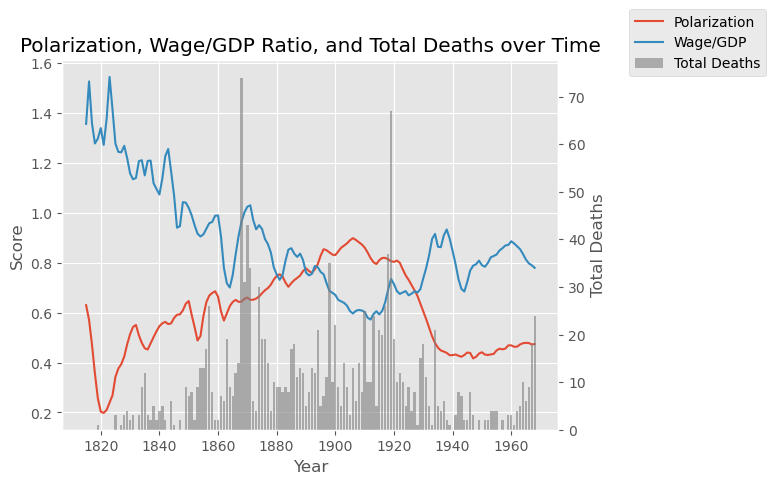
\includegraphics[keepaspectratio]{FInal_project_files/figure-pdf/cell-12-output-1.png}}

\pandocbounded{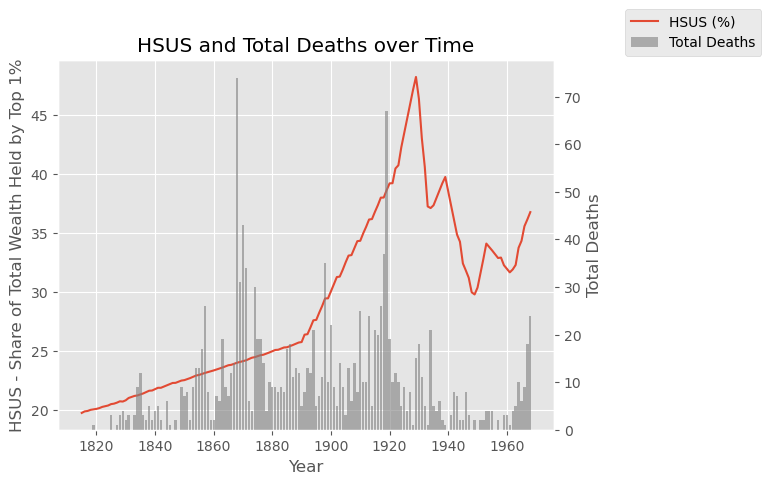
\includegraphics[keepaspectratio]{FInal_project_files/figure-pdf/cell-12-output-2.png}}

\pandocbounded{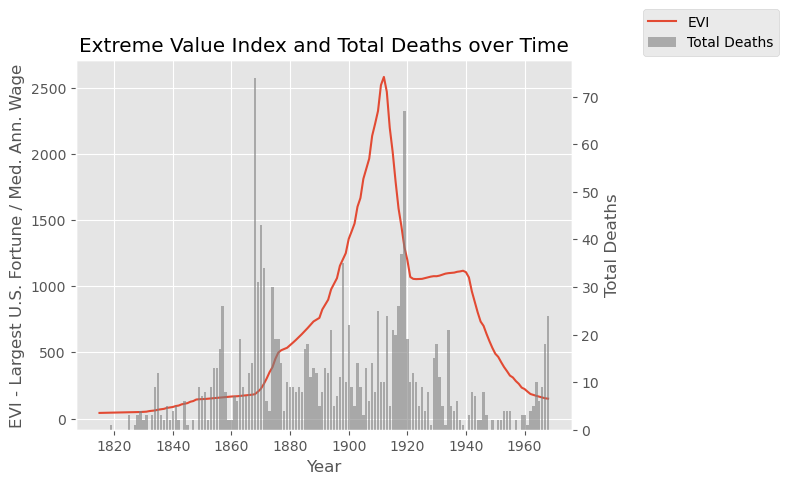
\includegraphics[keepaspectratio]{FInal_project_files/figure-pdf/cell-12-output-3.png}}

\begin{Shaded}
\begin{Highlighting}[]
\NormalTok{df.describe()}
\end{Highlighting}
\end{Shaded}

\begin{longtable}[]{@{}lllllllllllllllll@{}}
\toprule\noalign{}
& time & polarization & ratio & assassination & executions &
insurrection & lynching & mass suicide & rampage & riot & terrorism &
war & total\_deaths & Height(cm) & EVI & HSUS \\
\midrule\noalign{}
\endhead
\bottomrule\noalign{}
\endlastfoot
count & 154.000000 & 154.000000 & 154.000000 & 154.000000 & 154.0 &
154.0 & 154.000000 & 154.0 & 154.000000 & 154.000000 & 154.000000 &
154.000000 & 154.000000 & 154.000000 & 154.000000 & 154.000000 \\
mean & 1891.500000 & 0.603831 & 0.888165 & 0.279221 & 0.0 & 0.0 &
2.863636 & 0.0 & 0.123377 & 6.019481 & 0.038961 & 0.045455 & 9.370130 &
173.005306 & 643.338373 & 28.997821 \\
std & 44.600075 & 0.167190 & 0.215512 & 1.069462 & 0.0 & 0.0 & 4.584812
& 0.0 & 0.401434 & 7.201553 & 0.194133 & 0.287902 & 10.956212 & 2.805997
& 625.956548 & 7.210012 \\
min & 1815.000000 & 0.198197 & 0.572077 & 0.000000 & 0.0 & 0.0 &
0.000000 & 0.0 & 0.000000 & 0.000000 & 0.000000 & 0.000000 & 0.000000 &
169.131249 & 42.411092 & 19.764911 \\
25\% & 1853.250000 & 0.464987 & 0.735015 & 0.000000 & 0.0 & 0.0 &
0.000000 & 0.0 & 0.000000 & 1.000000 & 0.000000 & 0.000000 & 2.000000 &
170.775788 & 150.600303 & 22.852481 \\
50\% & 1891.500000 & 0.601311 & 0.839051 & 0.000000 & 0.0 & 0.0 &
1.000000 & 0.0 & 0.000000 & 4.000000 & 0.000000 & 0.000000 & 6.500000 &
172.537501 & 439.076486 & 26.414548 \\
75\% & 1929.750000 & 0.746655 & 0.989250 & 0.000000 & 0.0 & 0.0 &
4.000000 & 0.0 & 0.000000 & 8.000000 & 0.000000 & 0.000000 & 12.000000 &
175.795216 & 1067.298641 & 34.302688 \\
max & 1968.000000 & 0.898414 & 1.544620 & 11.000000 & 0.0 & 0.0 &
29.000000 & 0.0 & 2.000000 & 52.000000 & 1.000000 & 3.000000 & 74.000000
& 177.891684 & 2582.648997 & 48.226695 \\
\end{longtable}

\begin{Shaded}
\begin{Highlighting}[]
\NormalTok{df.isnull().}\BuiltInTok{sum}\NormalTok{()}
\end{Highlighting}
\end{Shaded}

\begin{verbatim}
time             0
polarization     0
ratio            0
assassination    0
executions       0
insurrection     0
lynching         0
mass suicide     0
rampage          0
riot             0
terrorism        0
war              0
total_deaths     0
Height(cm)       0
EVI              0
HSUS             0
dtype: int64
\end{verbatim}

\begin{Shaded}
\begin{Highlighting}[]
\CommentTok{\# List of columns to plot}
\NormalTok{columns\_to\_plot }\OperatorTok{=}\NormalTok{ df.columns.drop([}\StringTok{\textquotesingle{}time\textquotesingle{}}\NormalTok{])}

\CommentTok{\# Number of columns for subplots}
\NormalTok{n\_cols }\OperatorTok{=} \DecValTok{6}
\NormalTok{n\_rows }\OperatorTok{=}\NormalTok{ (}\BuiltInTok{len}\NormalTok{(columns\_to\_plot) }\OperatorTok{+}\NormalTok{ n\_cols }\OperatorTok{{-}} \DecValTok{1}\NormalTok{) }\OperatorTok{//}\NormalTok{ n\_cols}

\NormalTok{fig, axes }\OperatorTok{=}\NormalTok{ plt.subplots(n\_rows, n\_cols, figsize}\OperatorTok{=}\NormalTok{(}\DecValTok{15}\NormalTok{, n\_rows }\OperatorTok{*} \DecValTok{5}\NormalTok{))}

\ControlFlowTok{for}\NormalTok{ i, col }\KeywordTok{in} \BuiltInTok{enumerate}\NormalTok{(columns\_to\_plot):}
\NormalTok{    row }\OperatorTok{=}\NormalTok{ i }\OperatorTok{//}\NormalTok{ n\_cols}
\NormalTok{    col\_idx }\OperatorTok{=}\NormalTok{ i }\OperatorTok{\%}\NormalTok{ n\_cols}
\NormalTok{    sns.boxplot(data}\OperatorTok{=}\NormalTok{df[[col]], ax}\OperatorTok{=}\NormalTok{axes[row, col\_idx])}
\NormalTok{    axes[row, col\_idx].set\_title(}\SpecialStringTok{f\textquotesingle{}Boxplot of }\SpecialCharTok{\{}\NormalTok{col}\SpecialCharTok{\}}\SpecialStringTok{\textquotesingle{}}\NormalTok{)}

\CommentTok{\# Remove empty subplots}
\ControlFlowTok{for}\NormalTok{ j }\KeywordTok{in} \BuiltInTok{range}\NormalTok{(i }\OperatorTok{+} \DecValTok{1}\NormalTok{, n\_rows }\OperatorTok{*}\NormalTok{ n\_cols):}
\NormalTok{    fig.delaxes(axes.flatten()[j])}

\NormalTok{plt.tight\_layout()}
\NormalTok{plt.show()}
\end{Highlighting}
\end{Shaded}

\pandocbounded{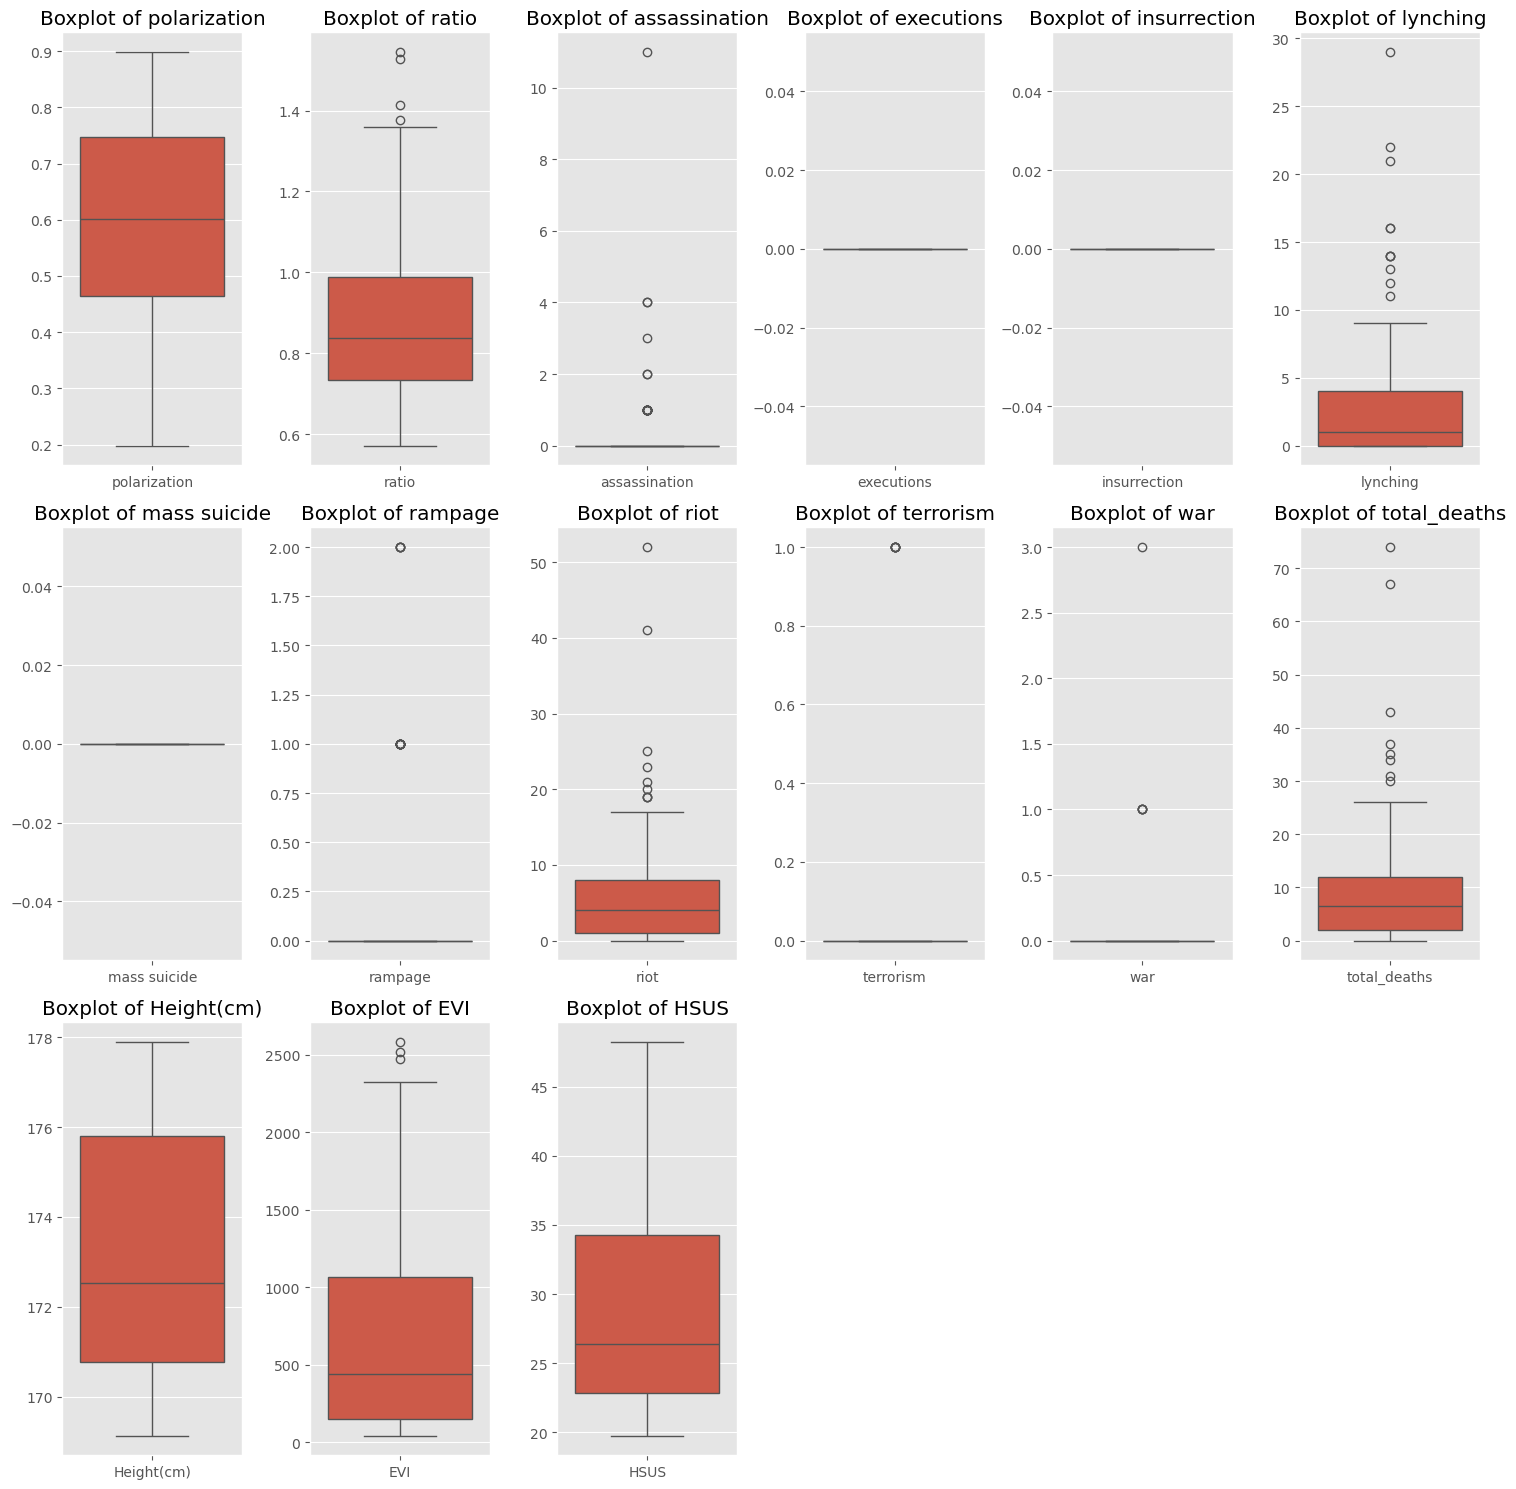
\includegraphics[keepaspectratio]{FInal_project_files/figure-pdf/cell-15-output-1.png}}

\begin{Shaded}
\begin{Highlighting}[]
\NormalTok{sns.pairplot(df)}
\NormalTok{plt.show()}
\end{Highlighting}
\end{Shaded}

\pandocbounded{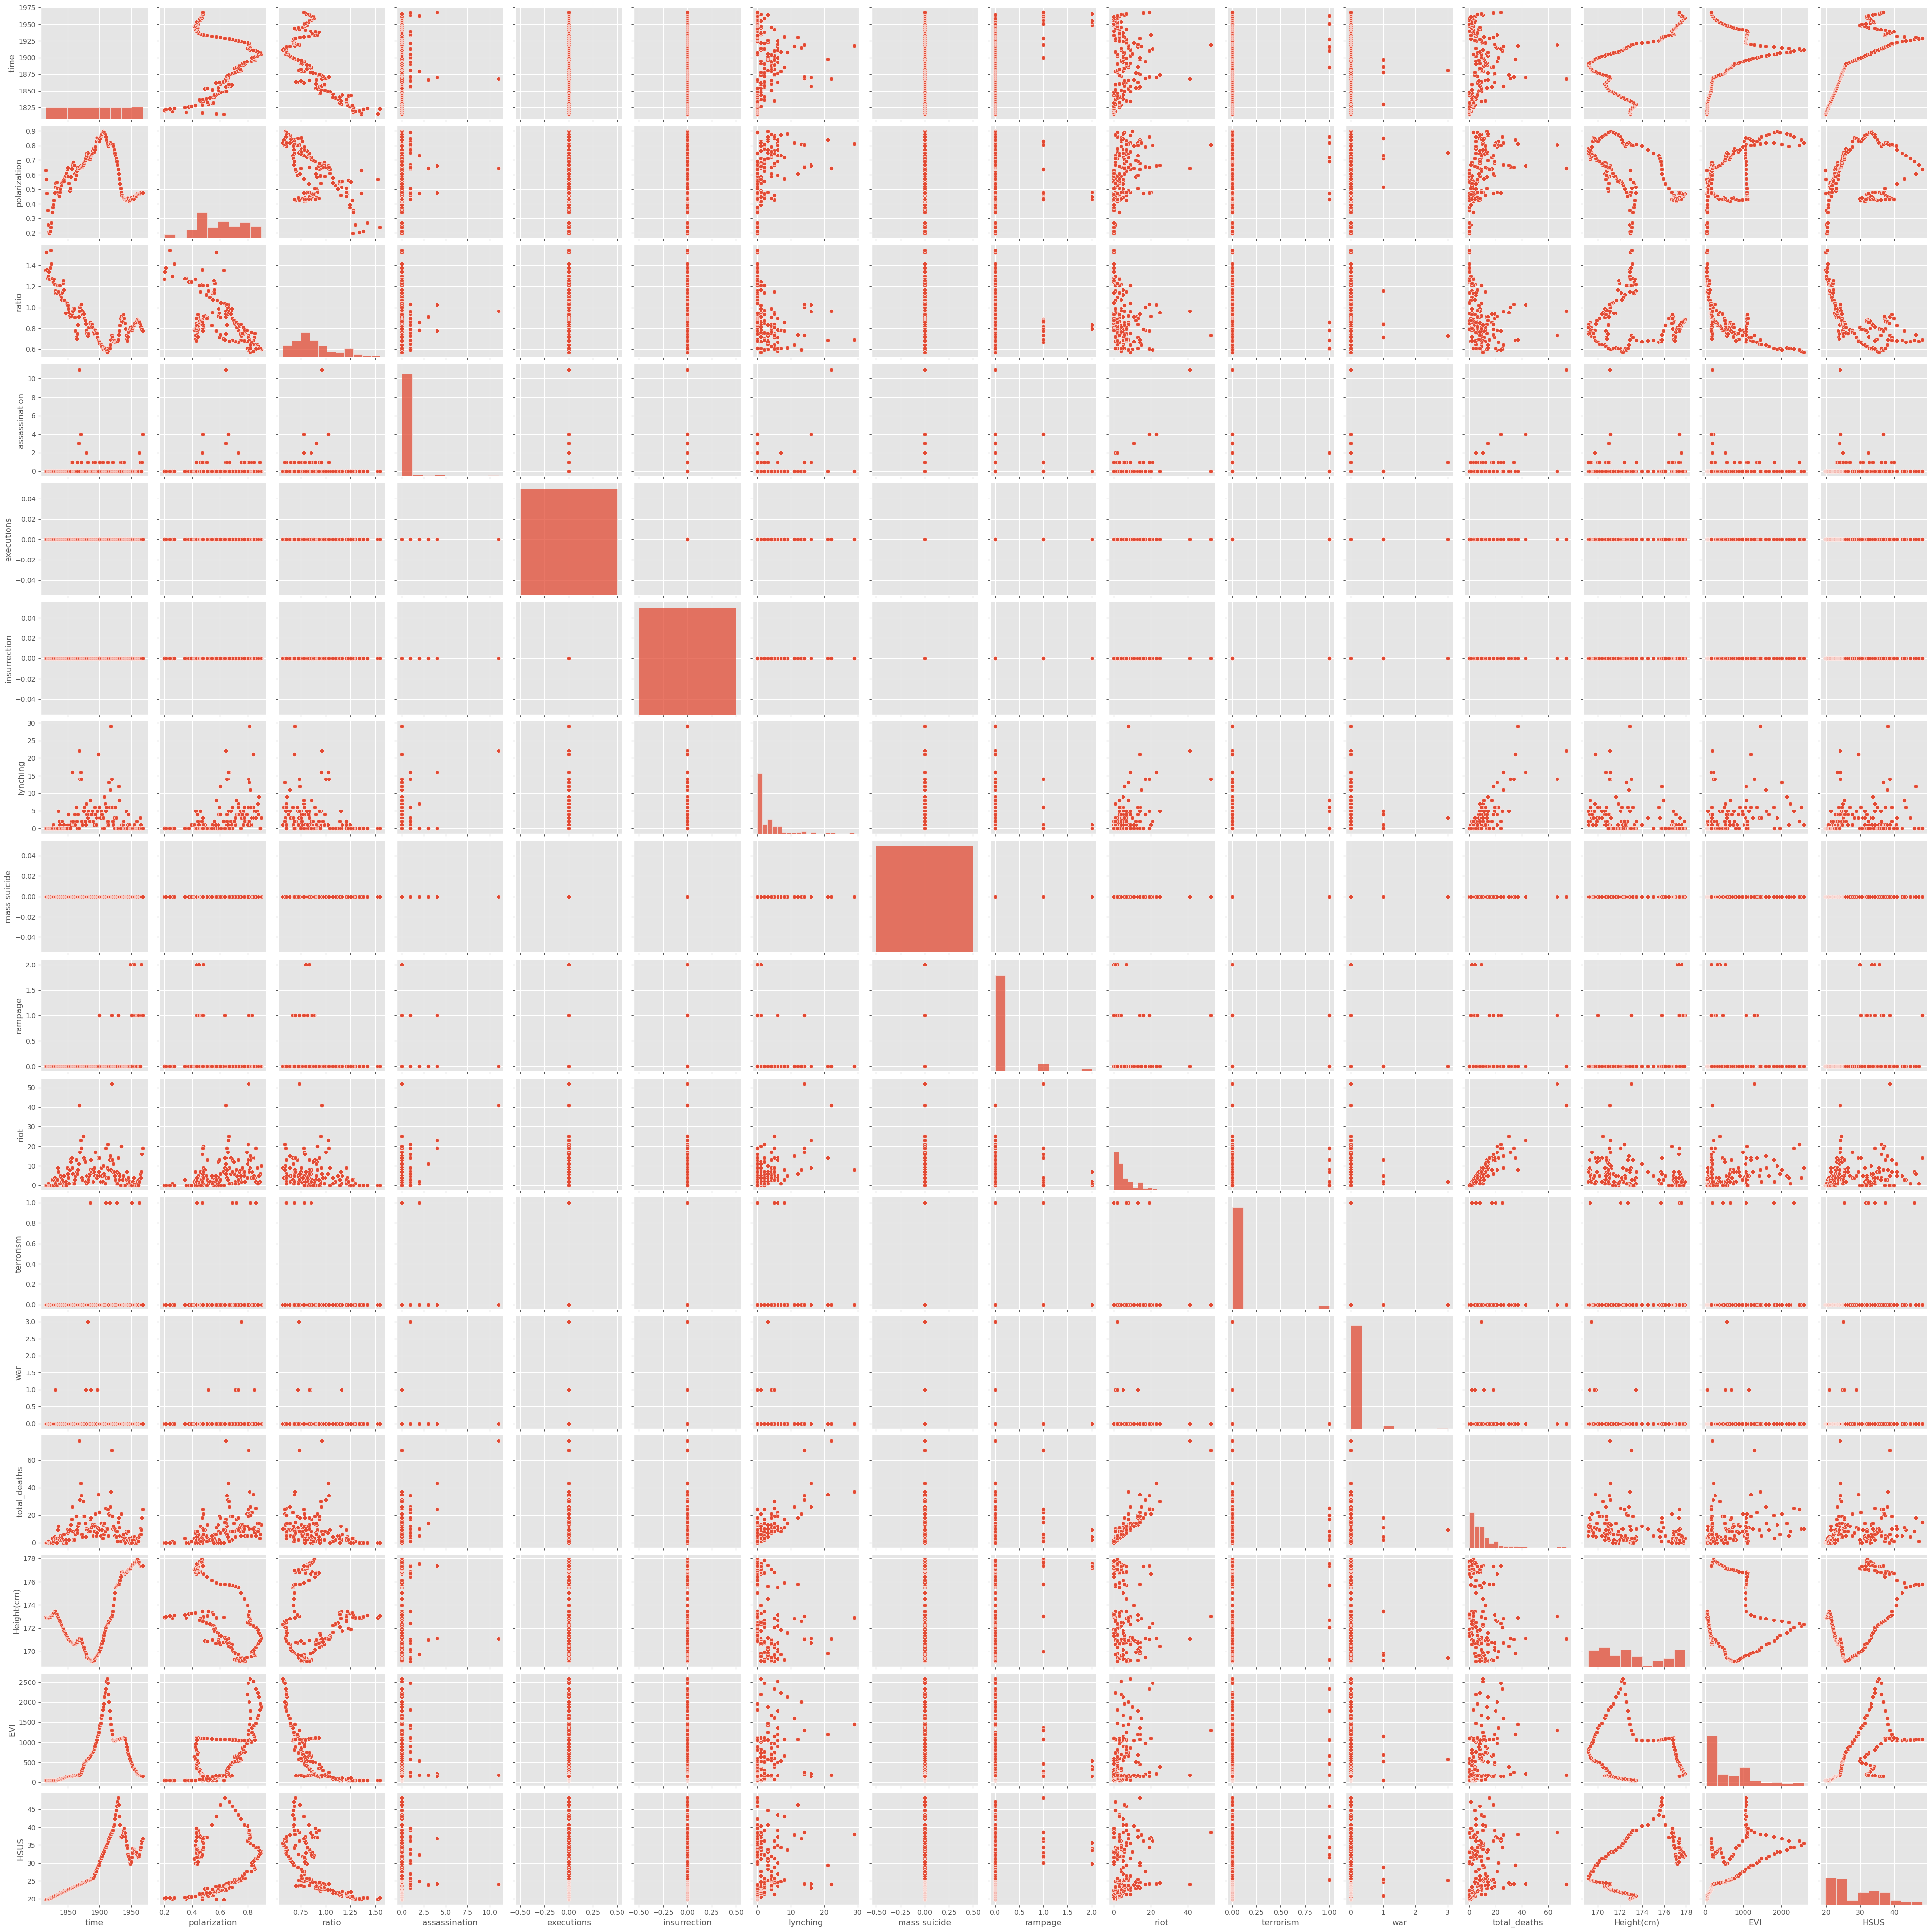
\includegraphics[keepaspectratio]{FInal_project_files/figure-pdf/cell-16-output-1.png}}

\begin{Shaded}
\begin{Highlighting}[]
\NormalTok{plt.figure(figsize}\OperatorTok{=}\NormalTok{(}\DecValTok{12}\NormalTok{, }\DecValTok{7}\NormalTok{))}
\NormalTok{sns.heatmap(df.corr(), annot}\OperatorTok{=}\VariableTok{True}\NormalTok{, cmap}\OperatorTok{=}\StringTok{\textquotesingle{}coolwarm\textquotesingle{}}\NormalTok{)}
\NormalTok{plt.title(}\StringTok{\textquotesingle{}Correlation Heatmap\textquotesingle{}}\NormalTok{)}
\NormalTok{plt.show()}
\end{Highlighting}
\end{Shaded}

\pandocbounded{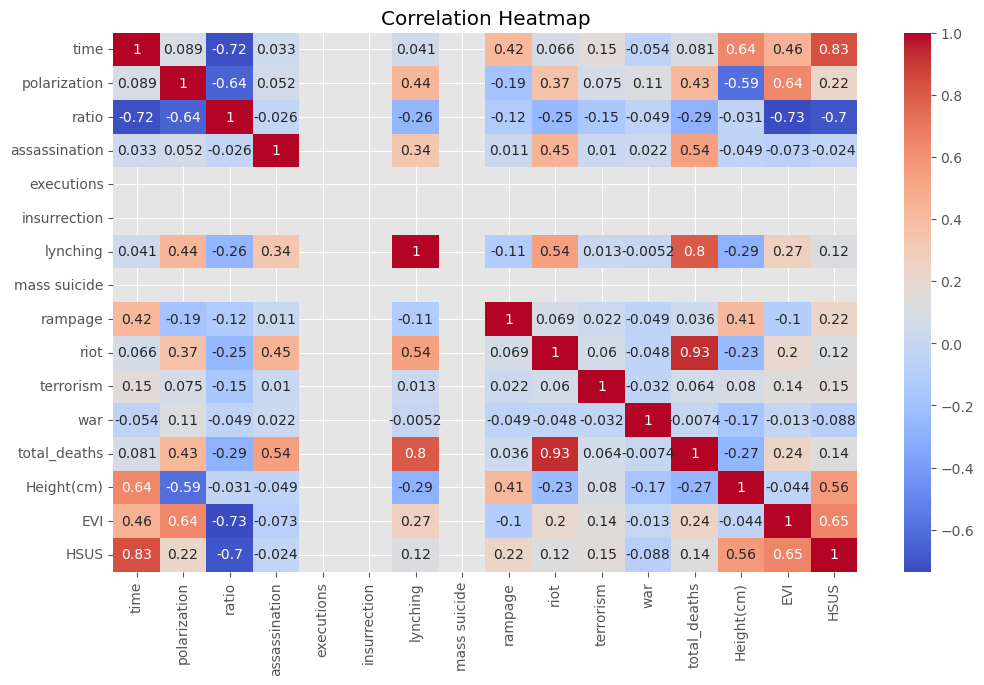
\includegraphics[keepaspectratio]{FInal_project_files/figure-pdf/cell-17-output-1.png}}

\subsection{Find the best regressor}\label{find-the-best-regressor}

Find the best regressor that would predict the instability index from
the various predictors. To be clear, you are asked to compare a limited
set of regressors of your choice -- not to identify the theoretically
optimal one.

\begin{itemize}
\tightlist
\item
  {[}x {]} Explain your modeling choices.
\item
  {[} x{]} Interpret any evaluation metrics you use.
\item
  {[} x{]} Summarize your conclusions in a short paragraph, i.e., the
  most interesting conclusion(s), the model that produced it, and how
  the model was chosen. You may include a figure if you find it helpful.
\end{itemize}

\begin{Shaded}
\begin{Highlighting}[]
\ImportTok{from}\NormalTok{ sklearn.model\_selection }\ImportTok{import}\NormalTok{ train\_test\_split}
\ImportTok{from}\NormalTok{ sklearn.preprocessing }\ImportTok{import}\NormalTok{ StandardScaler}
\ImportTok{from}\NormalTok{ sklearn.linear\_model }\ImportTok{import}\NormalTok{ LinearRegression, Ridge, Lasso}
\ImportTok{from}\NormalTok{ sklearn.ensemble }\ImportTok{import}\NormalTok{ RandomForestRegressor}
\ImportTok{from}\NormalTok{ sklearn.metrics }\ImportTok{import}\NormalTok{ mean\_squared\_error, mean\_absolute\_error, r2\_score}

\NormalTok{X }\OperatorTok{=}\NormalTok{ df.drop(columns}\OperatorTok{=}\NormalTok{[}\StringTok{"time"}\NormalTok{, }\StringTok{"total\_deaths"}\NormalTok{])  }
\NormalTok{y }\OperatorTok{=}\NormalTok{ df[}\StringTok{"total\_deaths"}\NormalTok{]}

\NormalTok{scaler }\OperatorTok{=}\NormalTok{ StandardScaler()}
\NormalTok{X\_scaled }\OperatorTok{=}\NormalTok{ scaler.fit\_transform(X)}

\NormalTok{X\_train, X\_test, y\_train, y\_test }\OperatorTok{=}\NormalTok{ train\_test\_split(X\_scaled, y, test\_size}\OperatorTok{=}\FloatTok{0.3}\NormalTok{, random\_state}\OperatorTok{=}\DecValTok{42}\NormalTok{)}

\NormalTok{models }\OperatorTok{=}\NormalTok{ \{}
    \StringTok{"Linear Regression"}\NormalTok{: LinearRegression(),}
    \StringTok{"Ridge Regression"}\NormalTok{: Ridge(alpha}\OperatorTok{=}\FloatTok{1.0}\NormalTok{),}
    \StringTok{"Lasso Regression"}\NormalTok{: Lasso(alpha}\OperatorTok{=}\FloatTok{0.1}\NormalTok{),}
    \StringTok{"Random Forest"}\NormalTok{: RandomForestRegressor(n\_estimators}\OperatorTok{=}\DecValTok{100}\NormalTok{, random\_state}\OperatorTok{=}\DecValTok{42}\NormalTok{)}
\NormalTok{\}}

\NormalTok{results }\OperatorTok{=}\NormalTok{ \{\}}

\ControlFlowTok{for}\NormalTok{ name, model }\KeywordTok{in}\NormalTok{ models.items():}
\NormalTok{    model.fit(X\_train, y\_train)}
\NormalTok{    y\_pred }\OperatorTok{=}\NormalTok{ model.predict(X\_test)}
\NormalTok{    results[name] }\OperatorTok{=}\NormalTok{ \{}
        \StringTok{"R2"}\NormalTok{: r2\_score(y\_test, y\_pred),}
        \StringTok{"MSE"}\NormalTok{: mean\_squared\_error(y\_test, y\_pred),}
        \StringTok{"MAE"}\NormalTok{: mean\_absolute\_error(y\_test, y\_pred)}
\NormalTok{    \}}

\NormalTok{results\_df }\OperatorTok{=}\NormalTok{ pd.DataFrame(results).T}
\NormalTok{results\_df}
\end{Highlighting}
\end{Shaded}

\begin{longtable}[]{@{}llll@{}}
\toprule\noalign{}
& R2 & MSE & MAE \\
\midrule\noalign{}
\endhead
\bottomrule\noalign{}
\endlastfoot
Linear Regression & 1.000000 & 2.552888e-29 & 3.420432e-15 \\
Ridge Regression & 0.999942 & 4.836788e-03 & 5.563760e-02 \\
Lasso Regression & 0.996825 & 2.632591e-01 & 2.519983e-01 \\
Random Forest & 0.942836 & 4.739526e+00 & 1.332553e+00 \\
\end{longtable}

After choosing 4 of the most used regressors(Linear, Ridge, Lasso and
random forest classifier) the models were trained and tested in order to
compare which one performed the best. The metrics used in order to
compare performance were R2 squared which explains variance, MSE whihc
penalizes larger errors heavily, so the lower score the better. Lastly
MAE was also used which essentially the lower the score the better.
Based on the results, Linear regression performed the best as it had the
highest \(R^2\), lowest mean squared error, and mean absolute error. The
performance was nearly perfect since it explained nearly 100 percent of
the variance in the instability index with little error. Because Linear
regression achieved such great results, complex models like Random
Forest were not necessary. Ridge and Lasso models performed well, yet
provided no advantage, confirming that feature redundancy and
multicollinearity were not concerns. Aditionally, the regressors were
tested with a smaller subset containing only 10 years which yielded
similar results. Linear Regression was still the best Performer.

\begin{Shaded}
\begin{Highlighting}[]
\NormalTok{models }\OperatorTok{=}\NormalTok{ results\_df.index}
\NormalTok{r2\_scores }\OperatorTok{=}\NormalTok{ results\_df[}\StringTok{\textquotesingle{}R2\textquotesingle{}}\NormalTok{]}

\NormalTok{plt.bar(models, r2\_scores, alpha}\OperatorTok{=}\FloatTok{0.7}\NormalTok{, color}\OperatorTok{=}\NormalTok{[}\StringTok{\textquotesingle{}blue\textquotesingle{}}\NormalTok{, }\StringTok{\textquotesingle{}green\textquotesingle{}}\NormalTok{, }\StringTok{\textquotesingle{}red\textquotesingle{}}\NormalTok{, }\StringTok{\textquotesingle{}orange\textquotesingle{}}\NormalTok{])}
\NormalTok{plt.xlabel(}\StringTok{"Regression Models"}\NormalTok{)}
\NormalTok{plt.ylabel(}\StringTok{"R² Score"}\NormalTok{)}
\NormalTok{plt.title(}\StringTok{"Model Performance Comparison)"}\NormalTok{)}
\NormalTok{plt.ylim(}\FloatTok{0.9}\NormalTok{, }\FloatTok{1.01}\NormalTok{) }
\NormalTok{plt.axhline(}\DecValTok{1}\NormalTok{, color}\OperatorTok{=}\StringTok{"black"}\NormalTok{, linewidth}\OperatorTok{=}\DecValTok{1}\NormalTok{, linestyle}\OperatorTok{=}\StringTok{"{-}{-}"}\NormalTok{, label}\OperatorTok{=}\StringTok{"Perfect Fit (R² = 1.0)"}\NormalTok{)}
\NormalTok{plt.legend()}
\NormalTok{plt.xticks(rotation}\OperatorTok{=}\DecValTok{15}\NormalTok{)}
\NormalTok{plt.show()}
\end{Highlighting}
\end{Shaded}

\pandocbounded{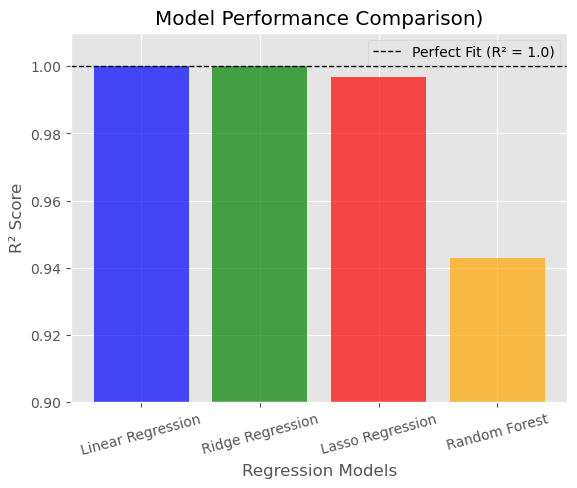
\includegraphics[keepaspectratio]{FInal_project_files/figure-pdf/cell-19-output-1.png}}

\subsection{Find the best dimensionality reduction for
regression}\label{find-the-best-dimensionality-reduction-for-regression}

You can restrict this part to reducing the data to two dimensions, to
three dimensions, or explore both options. You can test your variables
using the best regressor found in the previous section or a small number
of regressors (2-3 models at most).

\begin{itemize}
\tightlist
\item[$\square$]
  Explain modeling choices and evaluation metrics.
\item[$\square$]
  Summarize your conclusions in a short paragraph, i.e., the most
  interesting conclusion(s), the model that produced it, and how the
  model was chosen. You may include a figure if you find it helpful
\end{itemize}

\begin{Shaded}
\begin{Highlighting}[]
\ImportTok{from}\NormalTok{ sklearn.decomposition }\ImportTok{import}\NormalTok{ PCA}
\ImportTok{from}\NormalTok{ sklearn.feature\_selection }\ImportTok{import}\NormalTok{ SelectKBest, f\_regression}

\NormalTok{pca\_2d }\OperatorTok{=}\NormalTok{ PCA(n\_components}\OperatorTok{=}\DecValTok{2}\NormalTok{)}
\NormalTok{X\_pca\_2d }\OperatorTok{=}\NormalTok{ pca\_2d.fit\_transform(X\_scaled)}

\NormalTok{pca\_3d }\OperatorTok{=}\NormalTok{ PCA(n\_components}\OperatorTok{=}\DecValTok{3}\NormalTok{)}
\NormalTok{X\_pca\_3d }\OperatorTok{=}\NormalTok{ pca\_3d.fit\_transform(X\_scaled)}
\NormalTok{selector\_2d }\OperatorTok{=}\NormalTok{ SelectKBest(score\_func}\OperatorTok{=}\NormalTok{f\_regression, k}\OperatorTok{=}\DecValTok{2}\NormalTok{)}
\NormalTok{X\_sel\_2d }\OperatorTok{=}\NormalTok{ selector\_2d.fit\_transform(X\_scaled, y)}

\NormalTok{selector\_3d }\OperatorTok{=}\NormalTok{ SelectKBest(score\_func}\OperatorTok{=}\NormalTok{f\_regression, k}\OperatorTok{=}\DecValTok{3}\NormalTok{)}
\NormalTok{X\_sel\_3d }\OperatorTok{=}\NormalTok{ selector\_3d.fit\_transform(X\_scaled, y)}

\KeywordTok{def}\NormalTok{ evaluate\_reduced\_model(X\_reduced, name):}
\NormalTok{    X\_train\_r, X\_test\_r, y\_train\_r, y\_test\_r }\OperatorTok{=}\NormalTok{ train\_test\_split(X\_reduced, y, test\_size}\OperatorTok{=}\FloatTok{0.3}\NormalTok{, random\_state}\OperatorTok{=}\DecValTok{42}\NormalTok{)}
\NormalTok{    model }\OperatorTok{=}\NormalTok{ LinearRegression()}
\NormalTok{    model.fit(X\_train\_r, y\_train\_r)}
\NormalTok{    y\_pred\_r }\OperatorTok{=}\NormalTok{ model.predict(X\_test\_r)}
    
    \ControlFlowTok{return}\NormalTok{ \{}
        \StringTok{"Reduction Method"}\NormalTok{: name,}
        \StringTok{"R2 Score"}\NormalTok{: r2\_score(y\_test\_r, y\_pred\_r),}
        \StringTok{"MSE"}\NormalTok{: mean\_squared\_error(y\_test\_r, y\_pred\_r),}
        \StringTok{"MAE"}\NormalTok{: mean\_absolute\_error(y\_test\_r, y\_pred\_r)}
\NormalTok{    \}}

\NormalTok{results\_reduction }\OperatorTok{=}\NormalTok{ [}
\NormalTok{    evaluate\_reduced\_model(X\_pca\_2d, }\StringTok{"PCA (2D)"}\NormalTok{),}
\NormalTok{    evaluate\_reduced\_model(X\_pca\_3d, }\StringTok{"PCA (3D)"}\NormalTok{),}
\NormalTok{    evaluate\_reduced\_model(X\_sel\_2d, }\StringTok{"Feature Selection (Top 2)"}\NormalTok{),}
\NormalTok{    evaluate\_reduced\_model(X\_sel\_3d, }\StringTok{"Feature Selection (Top 3)"}\NormalTok{)}
\NormalTok{]}

\NormalTok{results\_reduction\_df }\OperatorTok{=}\NormalTok{ pd.DataFrame(results\_reduction)}
\NormalTok{results\_reduction\_df}
\end{Highlighting}
\end{Shaded}

\begin{longtable}[]{@{}lllll@{}}
\toprule\noalign{}
& Reduction Method & R2 Score & MSE & MAE \\
\midrule\noalign{}
\endhead
\bottomrule\noalign{}
\endlastfoot
0 & PCA (2D) & 0.075876 & 45.675370 & 5.380964 \\
1 & PCA (3D) & 0.838732 & 7.970765 & 2.142789 \\
2 & Feature Selection (Top 2) & 0.991761 & 0.407206 & 0.483158 \\
3 & Feature Selection (Top 3) & 0.996938 & 0.151351 & 0.283267 \\
\end{longtable}

\begin{Shaded}
\begin{Highlighting}[]
\NormalTok{plt.figure(figsize}\OperatorTok{=}\NormalTok{(}\DecValTok{8}\NormalTok{, }\DecValTok{5}\NormalTok{))}
\NormalTok{plt.bar(results\_reduction\_df[}\StringTok{"Reduction Method"}\NormalTok{], results\_reduction\_df[}\StringTok{"R2 Score"}\NormalTok{], alpha}\OperatorTok{=}\FloatTok{0.7}\NormalTok{, color}\OperatorTok{=}\NormalTok{[}\StringTok{\textquotesingle{}blue\textquotesingle{}}\NormalTok{, }\StringTok{\textquotesingle{}green\textquotesingle{}}\NormalTok{, }\StringTok{\textquotesingle{}red\textquotesingle{}}\NormalTok{, }\StringTok{\textquotesingle{}orange\textquotesingle{}}\NormalTok{])}
\NormalTok{plt.xlabel(}\StringTok{"Dimensionality Reduction Method"}\NormalTok{)}
\NormalTok{plt.ylabel(}\StringTok{"R² Score"}\NormalTok{)}
\NormalTok{plt.title(}\StringTok{"Comparison of Dimensionality Reduction Methods for Regression"}\NormalTok{)}
\NormalTok{plt.axhline(}\DecValTok{0}\NormalTok{, color}\OperatorTok{=}\StringTok{"black"}\NormalTok{, linewidth}\OperatorTok{=}\DecValTok{1}\NormalTok{, linestyle}\OperatorTok{=}\StringTok{"{-}{-}"}\NormalTok{)  }\CommentTok{\# Reference line at R² = 0}
\NormalTok{plt.xticks(rotation}\OperatorTok{=}\DecValTok{15}\NormalTok{)}
\NormalTok{plt.show()}
\end{Highlighting}
\end{Shaded}

\pandocbounded{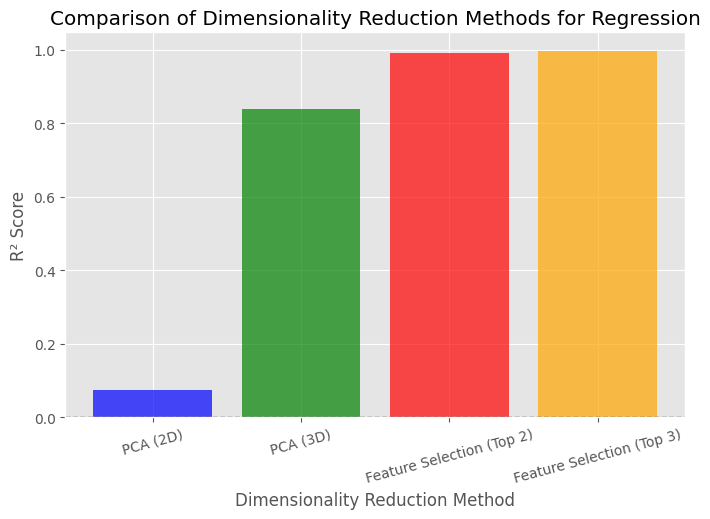
\includegraphics[keepaspectratio]{FInal_project_files/figure-pdf/cell-21-output-1.png}}

\begin{Shaded}
\begin{Highlighting}[]
\ImportTok{import}\NormalTok{ seaborn }\ImportTok{as}\NormalTok{ sns}
\NormalTok{final\_model }\OperatorTok{=}\NormalTok{ LinearRegression()}
\NormalTok{final\_model.fit(X\_sel\_3d, y)}
\NormalTok{coefficients }\OperatorTok{=}\NormalTok{ final\_model.coef\_}
\NormalTok{intercept }\OperatorTok{=}\NormalTok{ final\_model.intercept\_}
\NormalTok{selected\_features\_idx }\OperatorTok{=}\NormalTok{ selector\_3d.get\_support(indices}\OperatorTok{=}\VariableTok{True}\NormalTok{)}
\NormalTok{selected\_feature\_names }\OperatorTok{=}\NormalTok{ [df.columns[i }\OperatorTok{+} \DecValTok{1}\NormalTok{] }\ControlFlowTok{for}\NormalTok{ i }\KeywordTok{in}\NormalTok{ selected\_features\_idx]}

\NormalTok{equation }\OperatorTok{=} \SpecialStringTok{f"}\SpecialCharTok{\{}\NormalTok{intercept}\SpecialCharTok{:.2f\}}\SpecialStringTok{ "}  \CommentTok{\# Initialize the equation with the intercept}

\ControlFlowTok{for}\NormalTok{ coef, feature }\KeywordTok{in} \BuiltInTok{zip}\NormalTok{(coefficients, selected\_feature\_names):}
\NormalTok{    equation }\OperatorTok{+=} \SpecialStringTok{f"+ (}\SpecialCharTok{\{}\NormalTok{coef}\SpecialCharTok{:.2f\}}\SpecialStringTok{ * }\SpecialCharTok{\{}\NormalTok{feature}\SpecialCharTok{\}}\SpecialStringTok{) "}

\BuiltInTok{print}\NormalTok{(equation)}

\NormalTok{fig, axes }\OperatorTok{=}\NormalTok{ plt.subplots(}\DecValTok{1}\NormalTok{, }\DecValTok{3}\NormalTok{, figsize}\OperatorTok{=}\NormalTok{(}\DecValTok{15}\NormalTok{, }\DecValTok{5}\NormalTok{))}

\ControlFlowTok{for}\NormalTok{ i, feature }\KeywordTok{in} \BuiltInTok{enumerate}\NormalTok{(selected\_feature\_names):}
\NormalTok{    sns.regplot(x}\OperatorTok{=}\NormalTok{df[feature], y}\OperatorTok{=}\NormalTok{y, ax}\OperatorTok{=}\NormalTok{axes[i], scatter\_kws}\OperatorTok{=}\NormalTok{\{}\StringTok{\textquotesingle{}alpha\textquotesingle{}}\NormalTok{: }\FloatTok{0.7}\NormalTok{\}, line\_kws}\OperatorTok{=}\NormalTok{\{}\StringTok{"color"}\NormalTok{: }\StringTok{"red"}\NormalTok{\})}
\NormalTok{    axes[i].set\_xlabel(feature)}
\NormalTok{    axes[i].set\_ylabel(}\StringTok{"Instability Index"}\NormalTok{)}
\NormalTok{    axes[i].set\_title(}\SpecialStringTok{f"Linear Regression: }\SpecialCharTok{\{}\NormalTok{feature}\SpecialCharTok{\}}\SpecialStringTok{ vs Instability Index"}\NormalTok{)}

\NormalTok{plt.tight\_layout()}
\NormalTok{plt.show()}
\end{Highlighting}
\end{Shaded}

\begin{verbatim}
8.29 + (1.00 * assassination) + (4.29 * lynching) + (7.00 * riot) 
\end{verbatim}

\pandocbounded{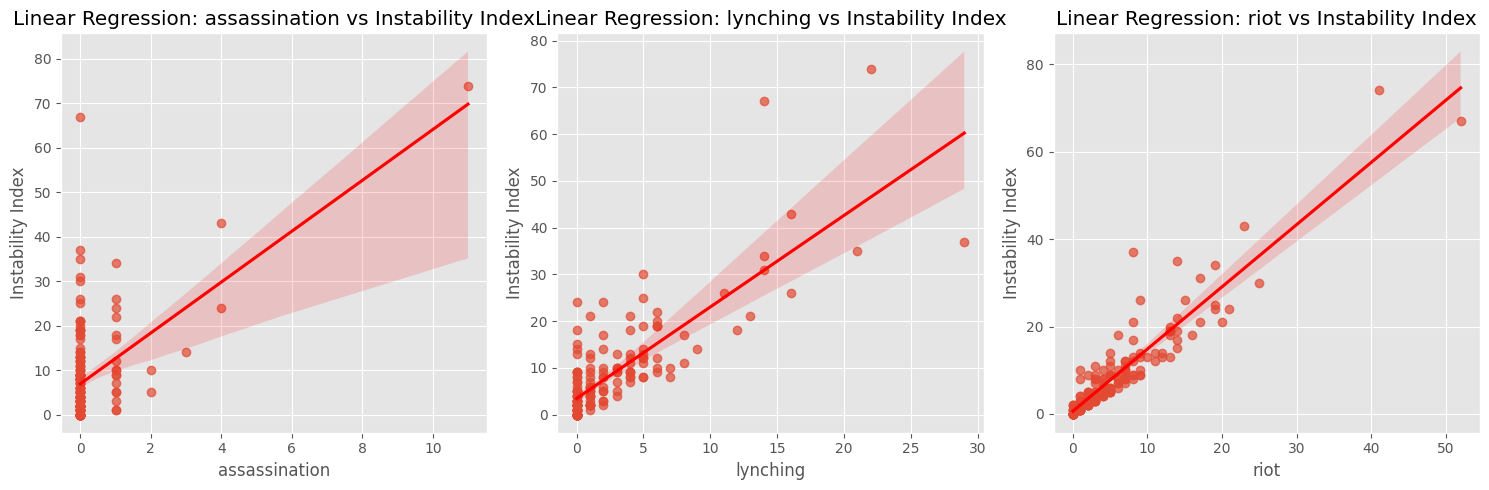
\includegraphics[keepaspectratio]{FInal_project_files/figure-pdf/cell-22-output-2.png}}

\begin{Shaded}
\begin{Highlighting}[]
\NormalTok{additional\_features }\OperatorTok{=}\NormalTok{ [}\StringTok{"EVI"}\NormalTok{, }\StringTok{"HSUS"}\NormalTok{]}
\NormalTok{selected\_feature\_names\_extended }\OperatorTok{=}\NormalTok{ selected\_feature\_names }\OperatorTok{+}\NormalTok{ additional\_features}

\NormalTok{fig, axes }\OperatorTok{=}\NormalTok{ plt.subplots(}\DecValTok{1}\NormalTok{, }\DecValTok{5}\NormalTok{, figsize}\OperatorTok{=}\NormalTok{(}\DecValTok{25}\NormalTok{, }\DecValTok{7}\NormalTok{))}

\ControlFlowTok{for}\NormalTok{ i, feature }\KeywordTok{in} \BuiltInTok{enumerate}\NormalTok{(selected\_feature\_names\_extended):}
\NormalTok{    sns.regplot(x}\OperatorTok{=}\NormalTok{df[feature], y}\OperatorTok{=}\NormalTok{y, ax}\OperatorTok{=}\NormalTok{axes[i], scatter\_kws}\OperatorTok{=}\NormalTok{\{}\StringTok{\textquotesingle{}alpha\textquotesingle{}}\NormalTok{: }\FloatTok{0.7}\NormalTok{\}, line\_kws}\OperatorTok{=}\NormalTok{\{}\StringTok{"color"}\NormalTok{: }\StringTok{"red"}\NormalTok{\})}
\NormalTok{    axes[i].set\_xlabel(feature)}
\NormalTok{    axes[i].set\_ylabel(}\StringTok{"Instability Index"}\NormalTok{)}
\NormalTok{    axes[i].set\_title(}\SpecialStringTok{f"Linear Regression: }\SpecialCharTok{\{}\NormalTok{feature}\SpecialCharTok{\}}\SpecialStringTok{ vs Instability Index"}\NormalTok{)}

\NormalTok{plt.tight\_layout()}
\NormalTok{plt.show()}
\end{Highlighting}
\end{Shaded}

\pandocbounded{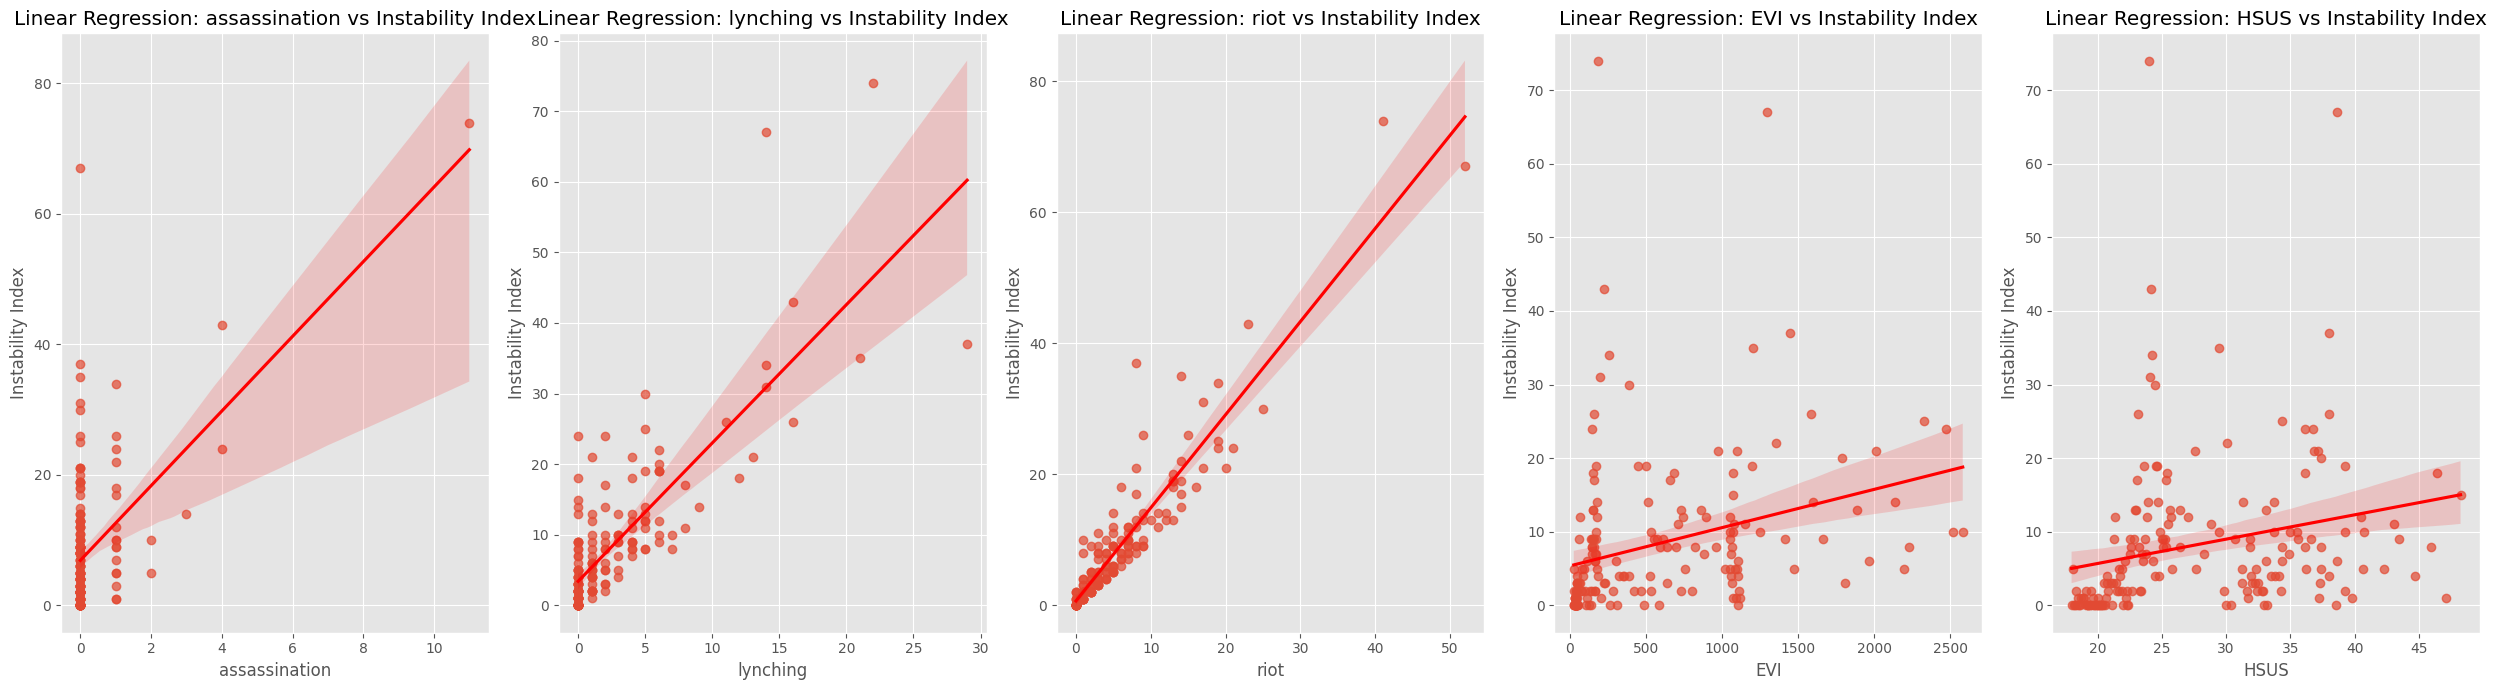
\includegraphics[keepaspectratio]{FInal_project_files/figure-pdf/cell-23-output-1.png}}

\begin{Shaded}
\begin{Highlighting}[]
\NormalTok{plt.figure(figsize}\OperatorTok{=}\NormalTok{(}\DecValTok{8}\NormalTok{, }\DecValTok{6}\NormalTok{))}
\NormalTok{plt.scatter(X\_pca\_2d[:, }\DecValTok{0}\NormalTok{], y, alpha}\OperatorTok{=}\FloatTok{0.7}\NormalTok{, label}\OperatorTok{=}\StringTok{"Data Points"}\NormalTok{, color}\OperatorTok{=}\StringTok{"blue"}\NormalTok{)}
\NormalTok{plt.xlabel(}\StringTok{"Principal Component 1"}\NormalTok{)}
\NormalTok{plt.ylabel(}\StringTok{"Instability Index"}\NormalTok{)}
\NormalTok{plt.title(}\StringTok{"PCA (2D)"}\NormalTok{)}
\NormalTok{plt.axhline(y}\OperatorTok{=}\NormalTok{np.mean(y), color}\OperatorTok{=}\StringTok{\textquotesingle{}red\textquotesingle{}}\NormalTok{, linestyle}\OperatorTok{=}\StringTok{\textquotesingle{}{-}{-}\textquotesingle{}}\NormalTok{, label}\OperatorTok{=}\StringTok{"Mean Instability Index"}\NormalTok{)}
\NormalTok{plt.legend()}
\NormalTok{plt.show()}
\end{Highlighting}
\end{Shaded}

\pandocbounded{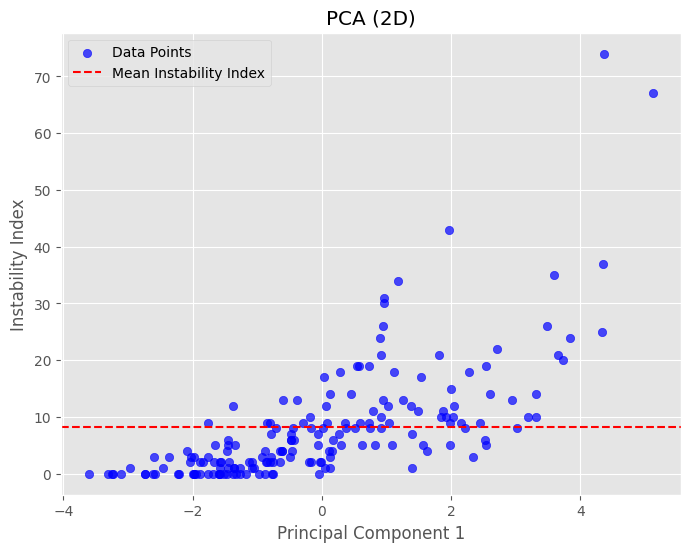
\includegraphics[keepaspectratio]{FInal_project_files/figure-pdf/cell-24-output-1.png}}

In order to compare dimensionality the choices used were PCA whichs
purpose was to capture the most variance in the data. Feature selection
was also implemented. The purpose of feature selection is to retain the
most relevant predictors based on significance. Similarly to the problem
above, R2 score, MSE, and MAE were used as metrics. After executing the
model, Feature selection with 3 features performed the best suggesting
keeping the main predictors yields better results. On the other hand PCA
performed poorly suggesting that important data is lost when performing
the model. Based on the results it is safe to say Linear regression with
selected features is the best option as it provides both
interpretability and superior regression performance.

\subsection{Find the best dimensionality reduction for unsupervised
classification}\label{find-the-best-dimensionality-reduction-for-unsupervised-classification}

Use only the predictor columns and not the outcome (instability) for
classification. You can restrict this part to reducing the data to two
dimensions, to three dimensions, or explore both options.

\begin{itemize}
\tightlist
\item[$\boxtimes$]
  You can test your variables using k-means or a small number of
  classifiers (2-3 models at most).
\item[$\square$]
  Explain modeling choices and evaluation metrics.
\item[$\square$]
  Summarize your conclusions in a short paragraph, i.e., the most
  interesting conclusion(s), the model that produced it, and how the
  model was chosen. You may include a figure if you find it helpful.
\end{itemize}

\begin{Shaded}
\begin{Highlighting}[]
\CommentTok{\# Dariel}

\ImportTok{from}\NormalTok{ sklearn.cluster }\ImportTok{import}\NormalTok{ KMeans}

\NormalTok{k\_values }\OperatorTok{=} \BuiltInTok{range}\NormalTok{(}\DecValTok{1}\NormalTok{, }\DecValTok{11}\NormalTok{)}
\NormalTok{inertia\_values }\OperatorTok{=}\NormalTok{ []}

\ControlFlowTok{for}\NormalTok{ k }\KeywordTok{in}\NormalTok{ k\_values:}
\NormalTok{    kmeans }\OperatorTok{=}\NormalTok{ KMeans(n\_clusters}\OperatorTok{=}\NormalTok{k, random\_state}\OperatorTok{=}\DecValTok{42}\NormalTok{)}
\NormalTok{    kmeans.fit(X\_scaled)}
\NormalTok{    inertia\_values.append(kmeans.inertia\_)}

\NormalTok{plt.figure()}
\NormalTok{plt.plot(k\_values, inertia\_values)}
\NormalTok{plt.xlabel(}\StringTok{\textquotesingle{}Number of k\textquotesingle{}}\NormalTok{)}
\NormalTok{plt.ylabel(}\StringTok{\textquotesingle{}Inertia\textquotesingle{}}\NormalTok{)}
\NormalTok{plt.title(}\StringTok{\textquotesingle{}Elbow Chart\textquotesingle{}}\NormalTok{)}
\NormalTok{plt.show()}
\end{Highlighting}
\end{Shaded}

\pandocbounded{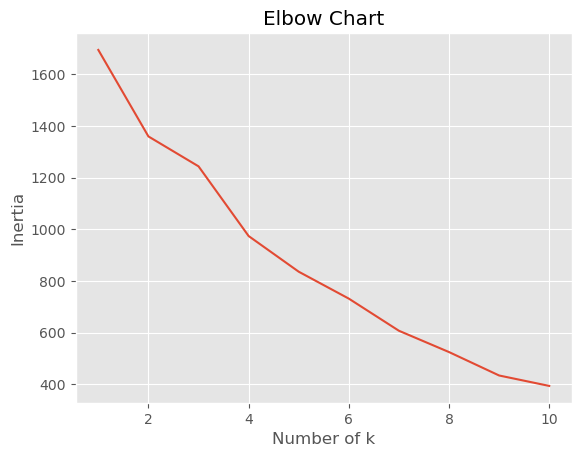
\includegraphics[keepaspectratio]{FInal_project_files/figure-pdf/cell-25-output-1.png}}

\begin{Shaded}
\begin{Highlighting}[]
\CommentTok{\# Dariel}

\ImportTok{from}\NormalTok{ sklearn.decomposition }\ImportTok{import}\NormalTok{ PCA}
\ImportTok{from}\NormalTok{ sklearn.metrics }\ImportTok{import}\NormalTok{ silhouette\_score}

\CommentTok{\# PCA reducing to 2 dimensions}
\NormalTok{pca\_2d }\OperatorTok{=}\NormalTok{ PCA(n\_components}\OperatorTok{=}\DecValTok{2}\NormalTok{)}
\NormalTok{X\_pca\_2d }\OperatorTok{=}\NormalTok{ pca\_2d.fit\_transform(X\_scaled)}

\CommentTok{\# PCA reducing to 3 dimensions}
\NormalTok{pca\_3d }\OperatorTok{=}\NormalTok{ PCA(n\_components}\OperatorTok{=}\DecValTok{3}\NormalTok{)}
\NormalTok{X\_pca\_3d }\OperatorTok{=}\NormalTok{ pca\_3d.fit\_transform(X\_scaled)}

\CommentTok{\#\#\#\#\#\#\#\#\#\#\#\#\#\#\#\#\#\#\#\#\#\#\#\#\#\#\#\#\#\#\#\#\#\#\#\#\#\#}
\CommentTok{\#     2D Clustering using K{-}Means    \#}
\CommentTok{\#\#\#\#\#\#\#\#\#\#\#\#\#\#\#\#\#\#\#\#\#\#\#\#\#\#\#\#\#\#\#\#\#\#\#\#\#\#}

\CommentTok{\# k=4; the elbow flattens around there}
\NormalTok{kmeans\_2d }\OperatorTok{=}\NormalTok{ KMeans(n\_clusters}\OperatorTok{=}\DecValTok{4}\NormalTok{, random\_state}\OperatorTok{=}\DecValTok{42}\NormalTok{)}
\NormalTok{clusters\_2d }\OperatorTok{=}\NormalTok{ kmeans\_2d.fit\_predict(X\_pca\_2d)}
\NormalTok{sil\_score\_2d }\OperatorTok{=}\NormalTok{ silhouette\_score(X\_pca\_2d, clusters\_2d)}

\BuiltInTok{print}\NormalTok{(}\StringTok{"PCA (2D) {-} Silhouette Score: }\SpecialCharTok{\{:.2f\}}\StringTok{"}\NormalTok{.}\BuiltInTok{format}\NormalTok{(sil\_score\_2d))}

\NormalTok{plt.figure(figsize}\OperatorTok{=}\NormalTok{(}\DecValTok{8}\NormalTok{,}\DecValTok{6}\NormalTok{))}
\NormalTok{plt.scatter(X\_pca\_2d[:, }\DecValTok{0}\NormalTok{], X\_pca\_2d[:, }\DecValTok{1}\NormalTok{], c}\OperatorTok{=}\NormalTok{clusters\_2d, cmap}\OperatorTok{=}\StringTok{\textquotesingle{}viridis\textquotesingle{}}\NormalTok{, alpha}\OperatorTok{=}\FloatTok{0.7}\NormalTok{)}
\NormalTok{plt.title(}\StringTok{"K{-}Means Clustering on PCA (2D)}\CharTok{\textbackslash{}n}\StringTok{Silhouette Score: }\SpecialCharTok{\{:.2f\}}\StringTok{"}\NormalTok{.}\BuiltInTok{format}\NormalTok{(sil\_score\_2d))}
\NormalTok{plt.xlabel(}\StringTok{"Principal Component 1"}\NormalTok{)}
\NormalTok{plt.ylabel(}\StringTok{"Principal Component 2"}\NormalTok{)}
\NormalTok{plt.colorbar(label}\OperatorTok{=}\StringTok{"Cluster Label"}\NormalTok{)}
\NormalTok{plt.show()}

\CommentTok{\#\#\#\#\#\#\#\#\#\#\#\#\#\#\#\#\#\#\#\#\#\#\#\#\#\#\#\#\#\#\#\#\#\#\#\#\#\#}
\CommentTok{\#    3D Clustering using K{-}Means     \#}
\CommentTok{\#\#\#\#\#\#\#\#\#\#\#\#\#\#\#\#\#\#\#\#\#\#\#\#\#\#\#\#\#\#\#\#\#\#\#\#\#\#}

\NormalTok{kmeans\_3d }\OperatorTok{=}\NormalTok{ KMeans(n\_clusters}\OperatorTok{=}\DecValTok{4}\NormalTok{, random\_state}\OperatorTok{=}\DecValTok{42}\NormalTok{)}
\NormalTok{clusters\_3d }\OperatorTok{=}\NormalTok{ kmeans\_3d.fit\_predict(X\_pca\_3d)}
\NormalTok{sil\_score\_3d }\OperatorTok{=}\NormalTok{ silhouette\_score(X\_pca\_3d, clusters\_3d)}

\BuiltInTok{print}\NormalTok{(}\StringTok{"PCA (3D) {-} Silhouette Score: }\SpecialCharTok{\{:.2f\}}\StringTok{"}\NormalTok{.}\BuiltInTok{format}\NormalTok{(sil\_score\_3d))}

\NormalTok{fig }\OperatorTok{=}\NormalTok{ plt.figure(figsize}\OperatorTok{=}\NormalTok{(}\DecValTok{8}\NormalTok{,}\DecValTok{10}\NormalTok{))}
\NormalTok{ax }\OperatorTok{=}\NormalTok{ fig.add\_subplot(}\DecValTok{111}\NormalTok{, projection}\OperatorTok{=}\StringTok{\textquotesingle{}3d\textquotesingle{}}\NormalTok{)}
\NormalTok{scatter }\OperatorTok{=}\NormalTok{ ax.scatter(X\_pca\_3d[:, }\DecValTok{0}\NormalTok{], X\_pca\_3d[:, }\DecValTok{1}\NormalTok{], X\_pca\_3d[:, }\DecValTok{2}\NormalTok{], }
\NormalTok{                     c}\OperatorTok{=}\NormalTok{clusters\_3d, cmap}\OperatorTok{=}\StringTok{\textquotesingle{}viridis\textquotesingle{}}\NormalTok{, alpha}\OperatorTok{=}\FloatTok{0.7}\NormalTok{)}
\NormalTok{ax.set\_title(}\StringTok{"K{-}Means Clustering on PCA (3D)}\CharTok{\textbackslash{}n}\StringTok{Silhouette Score: }\SpecialCharTok{\{:.2f\}}\StringTok{"}\NormalTok{.}\BuiltInTok{format}\NormalTok{(sil\_score\_3d))}
\NormalTok{ax.set\_xlabel(}\StringTok{"PC1"}\NormalTok{)}
\NormalTok{ax.set\_ylabel(}\StringTok{"PC2"}\NormalTok{)}
\NormalTok{ax.set\_zlabel(}\StringTok{"PC3"}\NormalTok{)}
\NormalTok{plt.legend(}\OperatorTok{*}\NormalTok{scatter.legend\_elements(), title}\OperatorTok{=}\StringTok{"Clusters"}\NormalTok{)}
\NormalTok{plt.show()}
\end{Highlighting}
\end{Shaded}

\begin{verbatim}
PCA (2D) - Silhouette Score: 0.54
\end{verbatim}

\pandocbounded{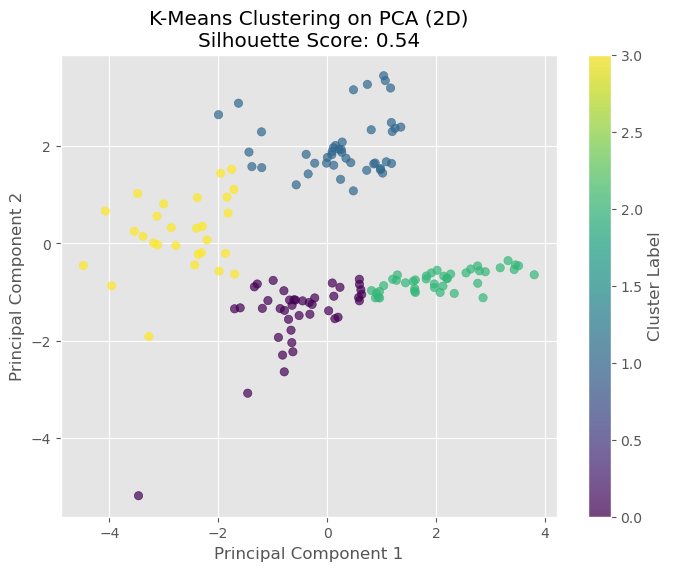
\includegraphics[keepaspectratio]{FInal_project_files/figure-pdf/cell-26-output-2.png}}

\begin{verbatim}
PCA (3D) - Silhouette Score: 0.45
\end{verbatim}

\pandocbounded{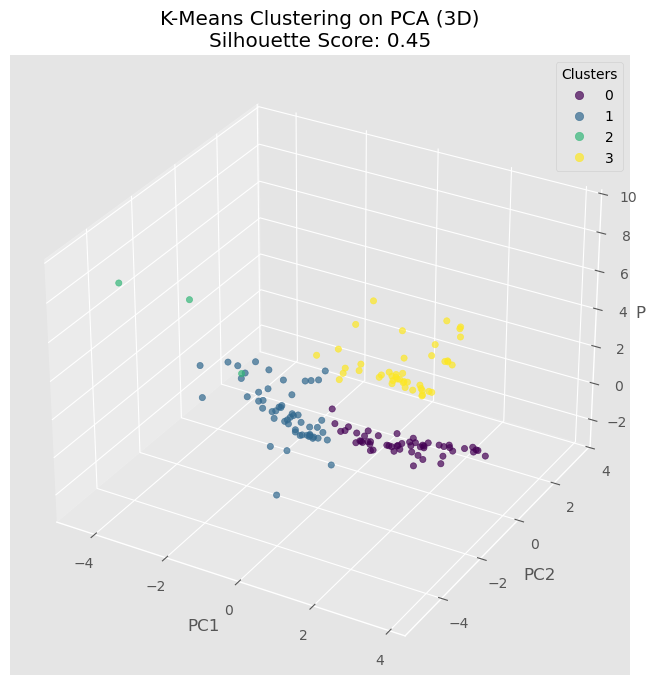
\includegraphics[keepaspectratio]{FInal_project_files/figure-pdf/cell-26-output-4.png}}

\subsection{Briefly explore the clusters of instability
scores}\label{briefly-explore-the-clusters-of-instability-scores}

Consider the cluster labels from the best clustering scheme from
previous section or from clustering using all/most of the original
features. Apply it to the corresponding records of the outcome column
(instability).

\begin{itemize}
\tightlist
\item[$\square$]
  Create a visualization of the results.
\item[$\square$]
  Summarize your conclusions. To be clear, the summary can be very
  short, and may be that the clusters do not exhibit any discernable or
  interpretable pattern. You may include a figure if you find it
  helpful.
\end{itemize}

\begin{Shaded}
\begin{Highlighting}[]
\CommentTok{\# Dariel}
\CommentTok{\#\#\#\#\#\#\#\#\#\#\#\#\#\#\#\#\#\#\#\#\#\#\#\#\#\#\#\#\#\#\#\#\#\#\#\#\#\#}
\CommentTok{\#     Clustering against outcome     \#}
\CommentTok{\#\#\#\#\#\#\#\#\#\#\#\#\#\#\#\#\#\#\#\#\#\#\#\#\#\#\#\#\#\#\#\#\#\#\#\#\#\#}
\CommentTok{\# \textquotesingle{}y\textquotesingle{} is the instability index}
\NormalTok{plt.figure(figsize}\OperatorTok{=}\NormalTok{(}\DecValTok{8}\NormalTok{,}\DecValTok{6}\NormalTok{))}
\NormalTok{sns.boxplot(x}\OperatorTok{=}\NormalTok{clusters\_2d, y}\OperatorTok{=}\NormalTok{y)}
\NormalTok{plt.xlabel(}\StringTok{"Cluster Label"}\NormalTok{)}
\NormalTok{plt.ylabel(}\StringTok{"Instability Index"}\NormalTok{)}
\NormalTok{plt.title(}\StringTok{"Instability Index by Cluster (PCA 2D + K{-}Means)"}\NormalTok{)}
\NormalTok{plt.show()}
\end{Highlighting}
\end{Shaded}

\pandocbounded{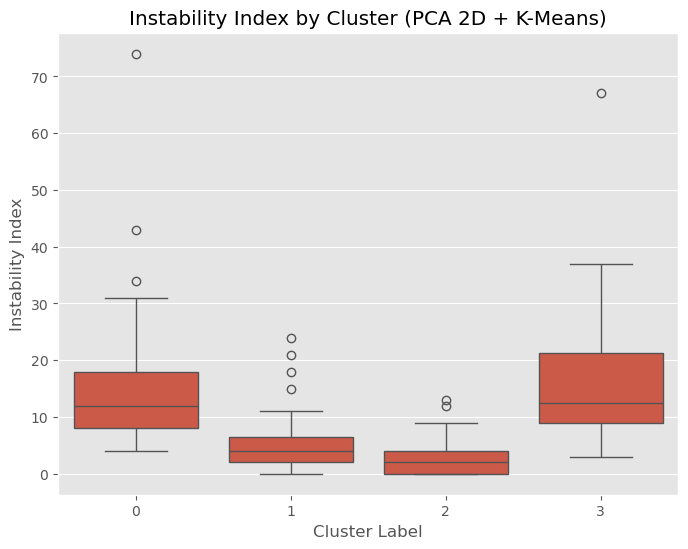
\includegraphics[keepaspectratio]{FInal_project_files/figure-pdf/cell-27-output-1.png}}

\subsection{Consider a real life modeling/prediction
problem}\label{consider-a-real-life-modelingprediction-problem}

\begin{itemize}
\tightlist
\item[$\square$]
  Try a large number (100? 1000?) different models
\item[$\square$]
  Examine their performances
\item[$\square$]
  Select the one that scores best on your performance metric of choice
\item[$\square$]
  Briefly discuss the potential disadvantage (or potential danger) of
  such and approach and how you might go about mitigating it.
\end{itemize}

\phantomsection\label{instability-index-by-cluster2}
\begin{Highlighting}
\textcolor{black}{NameError: name 'q7' is not defined}
\textcolor{black}{}\textcolor{QuartoInternalColor1}{---------------------------------------------------------------------------}\textcolor{QuartoInternalColor2}{}
\textcolor{QuartoInternalColor2}{}\textcolor{QuartoInternalColor1}{NameError}\textcolor{QuartoInternalColor2}{                                 Traceback (most recent call last)}
\textcolor{QuartoInternalColor2}{Cell }\textcolor{QuartoInternalColor3}{In[3], line 5}\textcolor{QuartoInternalColor2}{}
\textcolor{QuartoInternalColor2}{}\textcolor{QuartoInternalColor4}{      1}\textcolor{QuartoInternalColor2}{ }\textcolor{QuartoInternalColor9}{#| label: instability-index-by-cluster2}\textcolor{QuartoInternalColor2}{}
\textcolor{QuartoInternalColor2}{}\textcolor{QuartoInternalColor4}{      2}\textcolor{QuartoInternalColor2}{ }\textcolor{QuartoInternalColor9}{#| echo: false}\textcolor{QuartoInternalColor2}{}
\textcolor{QuartoInternalColor2}{}\textcolor{QuartoInternalColor4}{      3}\textcolor{QuartoInternalColor2}{ }\textcolor{QuartoInternalColor9}{#| fig-cap: "Instability Index by Cluster (PCA 2D + K-Means)"}\textcolor{QuartoInternalColor2}{}
\textcolor{QuartoInternalColor2}{}\textcolor{QuartoInternalColor3}{----> 5}\textcolor{QuartoInternalColor2}{ }\textcolor{QuartoInternalColor2}{q7}\textcolor{QuartoInternalColor2}{}
\textcolor{QuartoInternalColor2}{}\textcolor{QuartoInternalColor1}{NameError}\textcolor{QuartoInternalColor2}{: name 'q7' is not defined}
\end{Highlighting}

\begin{figure}

{\centering \pandocbounded{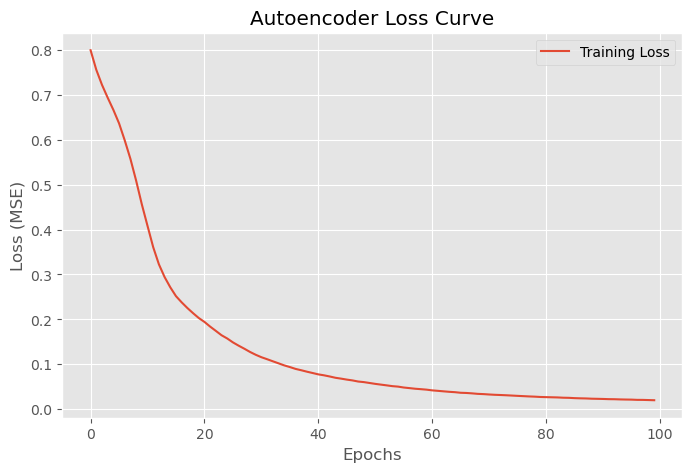
\includegraphics[keepaspectratio]{FInal_project_files/figure-pdf/autoencoder-loss-curve-output-1.png}}

}

\caption{The loss curve of the autoencoder model.}

\end{figure}%

\begin{figure}

{\centering \pandocbounded{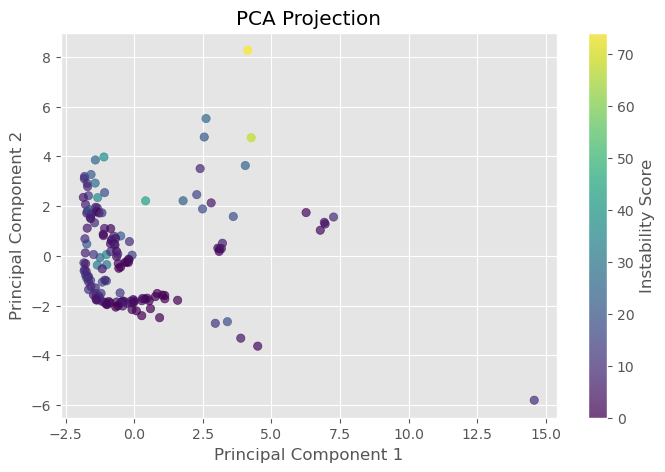
\includegraphics[keepaspectratio]{FInal_project_files/figure-pdf/pca-projection-output-1.png}}

}

\caption{PCA projection of the latent space.}

\end{figure}%

The results show that linear models (Linear Regression, Ridge, Lasso)
performed best, with near-perfect R² scores, suggesting a strong linear
relationship in the data---but also raising concerns about overfitting
or data leakage. Tree-based models (Random Forest, Decision Trees,
Gradient Boosting) had mixed performance, sometimes scoring well but
also showing high error and instability, likely due to sensitivity to
hyperparameters or feature selection issues. The wide range of results
highlights the risk of blindly testing a large number of models
(100-1000) without proper validation. Some models perform well by chance
rather than true predictive power. To mitigate overfitting and
instability, cross-validation, hyperparameter tuning, and feature
selection are crucial. While testing many models helps identify strong
candidates, efficient selection and proper validation matter more than
force experimentation like training 100 models. Using an autoencoder for
this part was helpful since it reduced the high-dimensional feature
space into a more compact representation, helping models focus on the
most relevant patterns rather than redundant data. it also reduced time
consumption by compressing the data in an optimal way.




\end{document}
